\documentclass[class=article,crop=false]{standalone}
\usepackage{amsmath}
\usepackage{xcolor}
\usepackage{mhchem}
\usepackage[subpreambles=true]{standalone}
\begin{document}
\lecture
\section{Quantum Harmonic Oscillator}
Consider a classical simple harmonic oscillator. For example, a block with mass m, attached to a spring with constant k, oscillates about its equilibrium on a frictionless surface. The force exerted by the spring is F = -kx. The elastic potential energy is $U = 1/2\ kx^2$. \\

From Newton's laws, the motion of th eclassical oscillator is shown to have an angular frequency $\omega_0$ and period T given by:
$$ \omega_0 = \sqrt{\frac{k}{m}}\ \ \ T = 2\pi \sqrt{\frac{m}{k}} $$

The quantum mechanical version of this system \\

In nature many systems behave \emph{approximately} as a quantum oscillator, for example a vibrating diatomic molecule. \\

The Schrödinger equation:
$$ - \frac{\bar{h}^2}{2m} \frac{d^2\psi}{dx^2} + 1/2\ kx^2 \psi(x) = E\psi(x) $$

Here, no boundaries between regions of different potential energy apply. For x approaches positive or negative infinity, the wave function must vanish. Simlplest function satisfying this (which will be the ground state!):
$$\psi(x) = Ae^{-ax^2} $$
Where a, A are constants.\\

Let's find the constants a, A:
$$ \frac{d\psi}{dx} = A(-2ax)e^{-ax^2} $$
$$ \frac{d^2\psi}{dx^2} = A(-2a)e^{-ax^2} + A(-2ax)e^{-ax^2} $$
$$ \frac{d^2\psi}{dx^2} = A(-2a)e^{-ax^2} + A(-2ax)^2e^{-ax^2} $$

Substitute into Schrödinger equation:
$$ - \frac{\bar{h}^2}{2m} 2a(-2ax^2 - 1)Ae^{-ax^2} + 1/2\ kx^2 A(-2ax)e^{-ax^2} = E\psi(x) $$
The exponentials cancel out on both sides of the equation.
$$ - \frac{a\bar{h}^2}{m} (2ax^2 - 1) + 1/2 kx^2 = E $$
We want a solution that is valid for ANY value of x:
$$ \left( \frac{k}{2} - \frac{2a^2\bar{h}^2}{m}\right) x^2 = E - \frac{a\bar{h}^2}{2} $$
Each side must be equal to zero
$$ \frac{k}{2} - \frac{2a^2\bar{h}^2}{m} = 0 \rightarrow a = \frac{\sqrt{km}}{2\bar{h}} $$

$$ E - \frac{a\bar{h}^2}{m} = 0 \rightarrow E - \frac{a\bar{h}}{m} = \frac{\bar{h}}{2} \sqrt{\frac{k}{m}} $$

Write energy in terms of classical angular frequency:
$$ \omega_0 = blah $$

The ground state wave function for our quantum oscillator is now:
$$ \psi(x) = A e^{-ax^2}\ for\ a = \frac{\sqrt{km}}{2\bar{h}} $$
We can find the constant A by normalization, yielding:
$$ \psi(x) = \left(\frac{m \omega_0}{\bar{h}\pi} \right)^{1/3} e^{-\sqrt{km}/2\bar{h}x^2} $$

The \emph{general} solutions is more involved:
$$ \psi_n(x) = A\ fn(x) e^{-ax^2} $$
Where $f_n(x)$: a polynomial with highest power of x is $x^n$.

The corresponding energies will be:
$$ E_n = \left(n + \frac{1}{2}\right)\bar{h} \omega_0 \ \ \ n=0,1,2,...$$


\begin{figure}[h!]
	\centering
	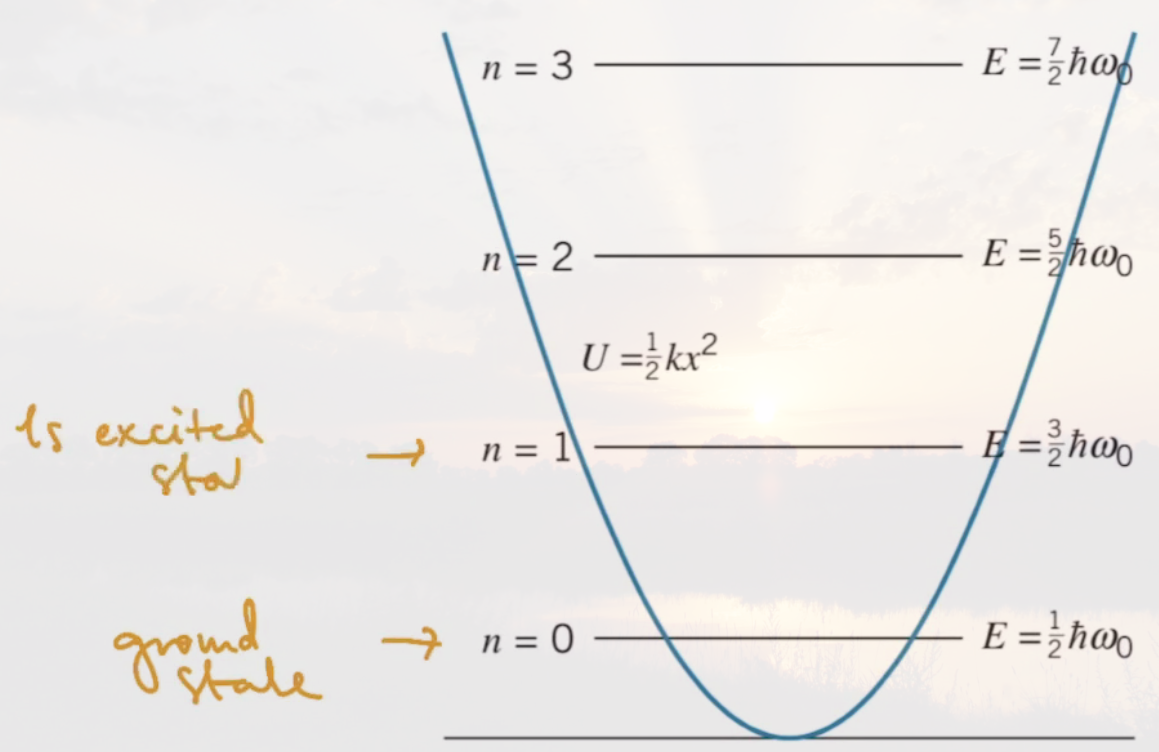
\includegraphics[width=.8\linewidth]{./Images/energies.png}
	\caption{This describes the ground state, 1st excited state, etc.}
\end{figure}

\subsection{Harmonic Oscillator \& Probabilities}
The below shows the probability density for a few different states for the quantum oscillator. The dashed lines show the classical probabilities for the equivalent energies.\\

Note: Probabilities extend beyond the classical region! And, distance between the classical turning points increases with increasing energy.

\begin{figure}[h!]
	\centering
	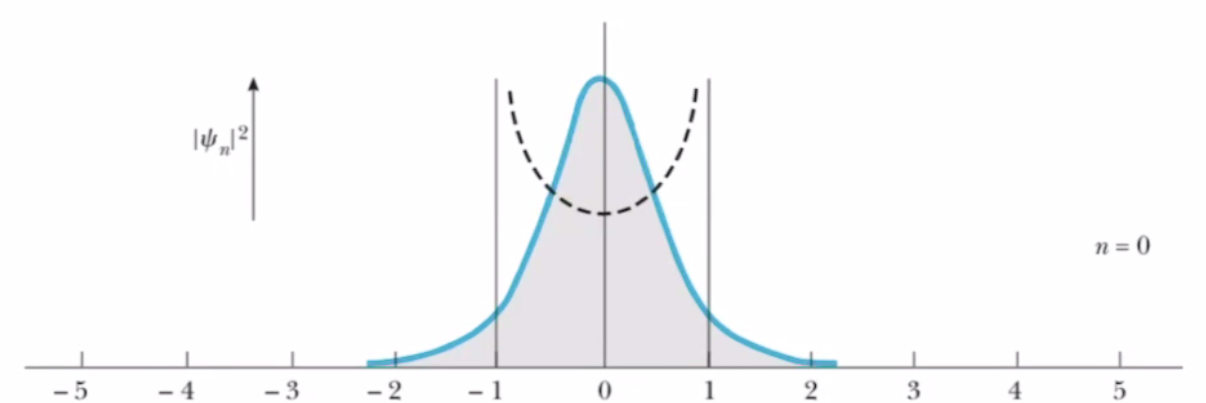
\includegraphics[width=.8\linewidth]{./Images/quantum_harmonic.png}
	\caption{We have a non-zero probability to find the particle in the forbidden region}
\end{figure}

\begin{figure}[h!]
	\centering
	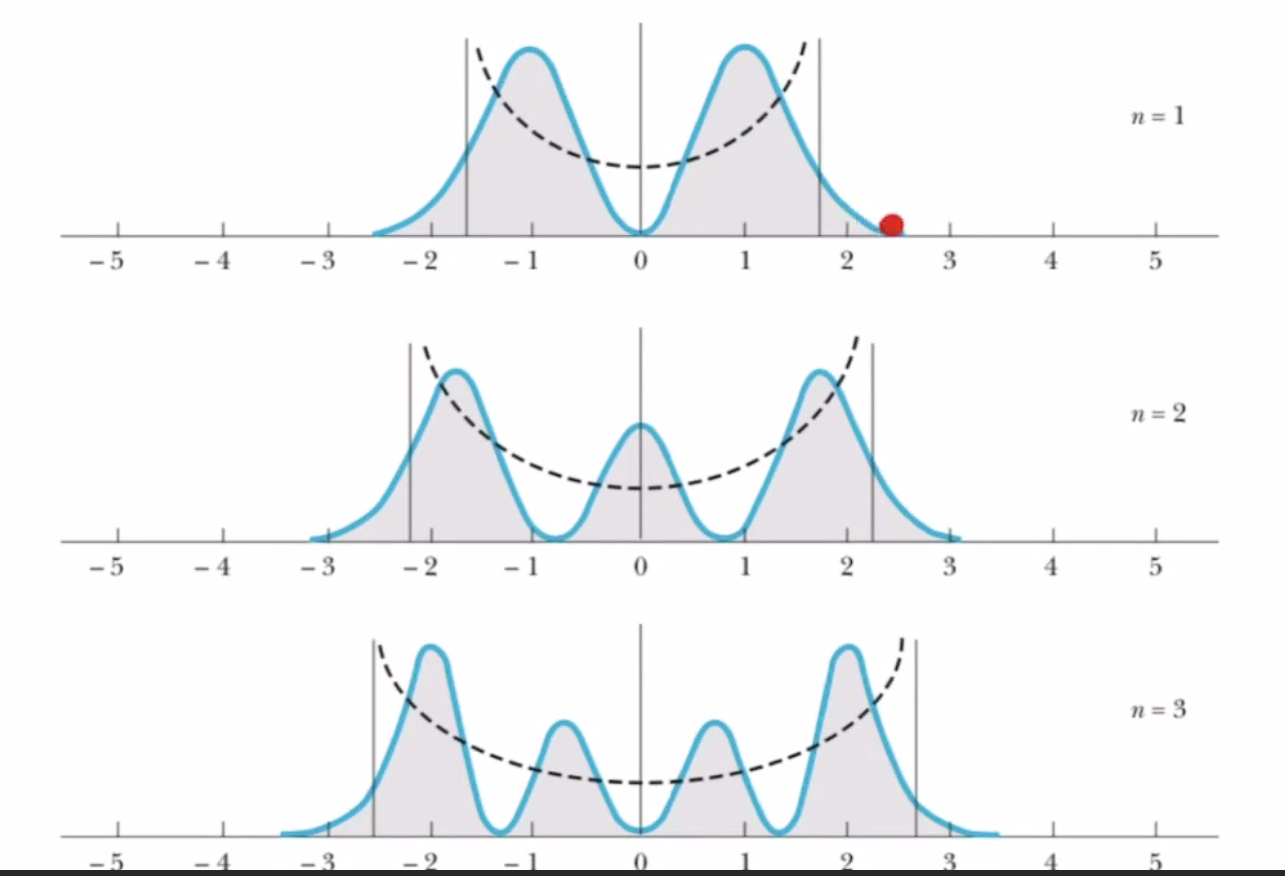
\includegraphics[width=.8\linewidth]{./Images/quantum_harmonic_2.png}
	\caption{We have a non-zero probability to find the particle in the forbidden region}
\end{figure}

\newpage
\section{Potential Energy Steps}
\subsection{Where E $>$ U}
In the following we will se what happens when a particle moves (in one dimension) from a region of constant potential energy to a region with a different potential energy.


\begin{figure}[h!]
	\centering
	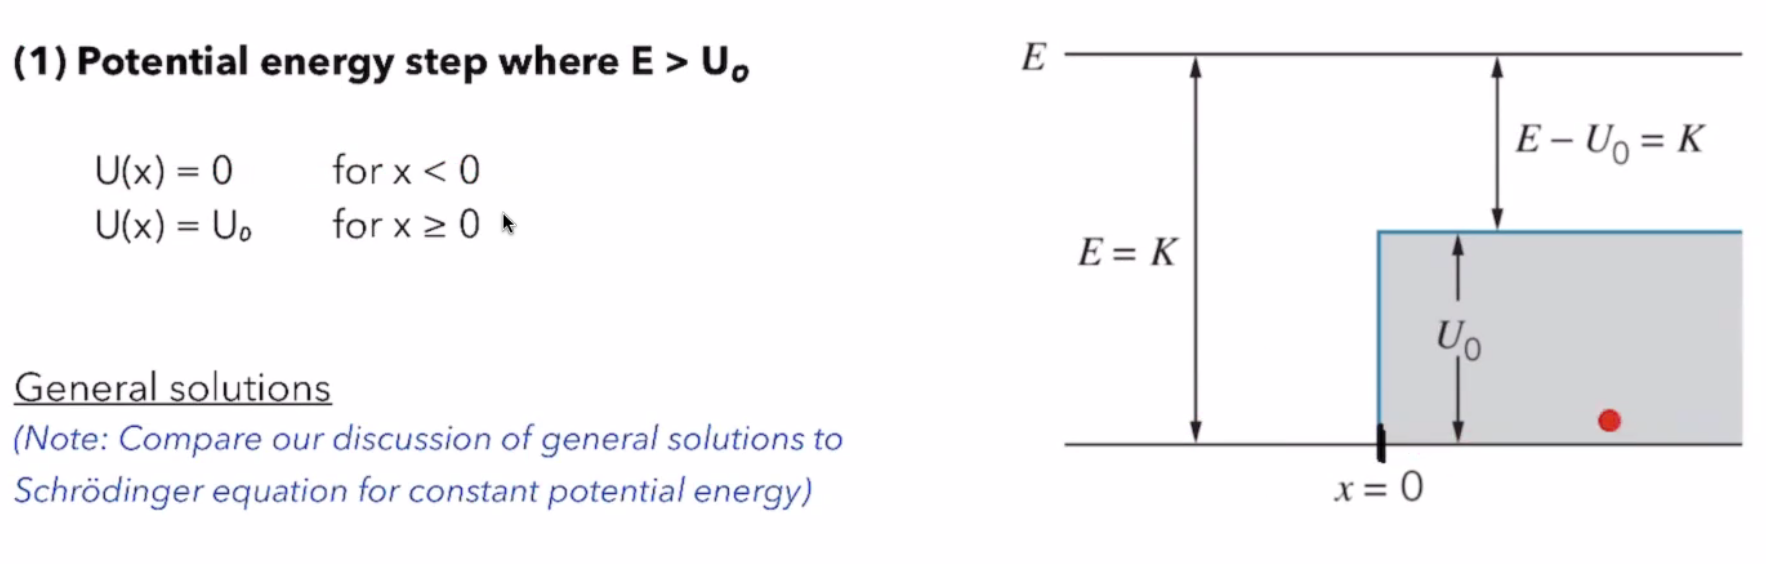
\includegraphics[width=1\linewidth]{./Images/pe_steps.png}
	\caption{Greater potential on the right side.}
\end{figure}

General solutions:
$$ For\ x<0: \psi_0(x) = A\ sin(k_0x) + B\ cos(k_0x)\ \ \ k_0 = \sqrt{\frac{2mE}{\bar{h}^2}} $$
$$ For\ x\geq0: \psi_1(x) = A\ sin(k_1x) + B\ cos(k_1x)\ \ \ k_1 = \sqrt{\frac{2m(U_0-E)}{\bar{h}^2}} $$

It is convenient to write these in terms of Complex Exponentials instead. We also want to introduce time-dependence!
$$ x < 0:\ \Psi_0(x,t) = A'e^{i(k_0x-\omega t)} + B'e^{-i(k_0x+\omega t)} $$
$$ x \geq 0:\ \Psi_1(x,t) = C'e^{i(k_1x-\omega t)} + D'e^{-i(k_1x+\omega t)} $$
Where A', B', C', D' are constants that we would need to determine.

We can think of this as a sum of waves; positive e term in the positive x-direction and the negative e term in the negatvie x-direction. The squared magnitude of each coefficient gives the intensity of hte corresponding component wave.


\begin{figure}[h!]
	\centering
	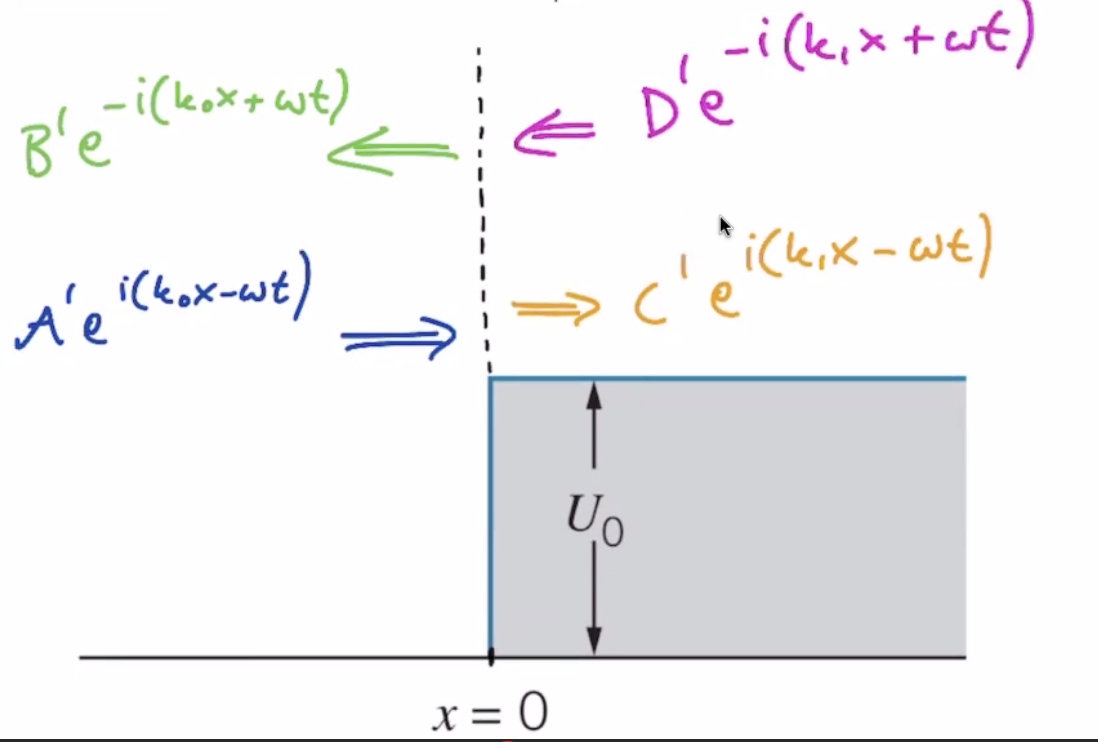
\includegraphics[width=1\linewidth]{./Images/ref_tra_comp.png}
	\caption{We can think of this as reflected and transmitted compontents. The blue wave is the incident wave, with the green wave the component that is reflected. The orange wave is the wave that is transmitted, and the purple wave must be zero.}
\end{figure}

If we are describiing particles moving from the left to the potential energy step:
$ D' = 0 $ \\
$ |A'|^2 $= intensity of incident wave \\
$ |B'|^2 $= intensity of reflected wave \\
$ |C'|^2 $= intensity of transmitted wave \\

From this we can say something about the fraction that is reflected vs transmitted:\\
Fraction reflected :
$$ \frac{|B'|^2}{|A'|^2} $$
Fraction transmitted :
$$ \frac{|C'|^2}{|A'|^2} $$
The sum must be 1.

\subsubsection{Probability Density}

\begin{figure}[h!]
	\centering
	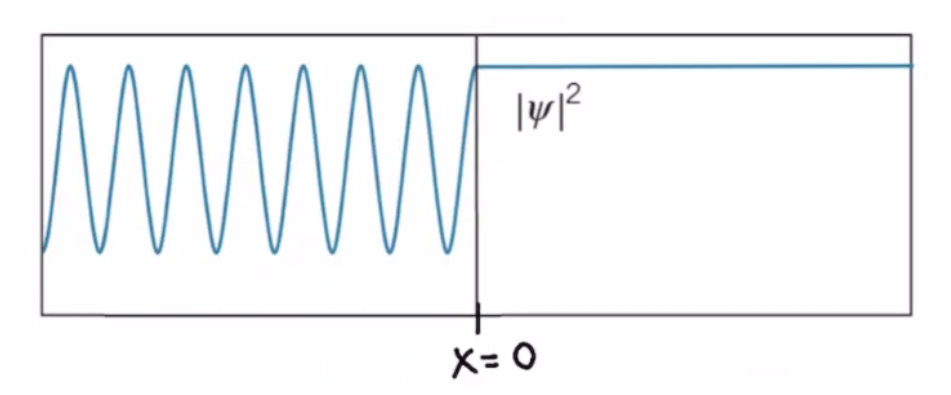
\includegraphics[width=0.6\linewidth]{./Images/probability_density.png}
	\caption{There is an oscillating behavior to the left of the boundary, which is caused by an interference between the incident and reflected wave.}
\end{figure}

\subsection{Where E $<$ U}

\begin{figure}[h!]
	\centering
	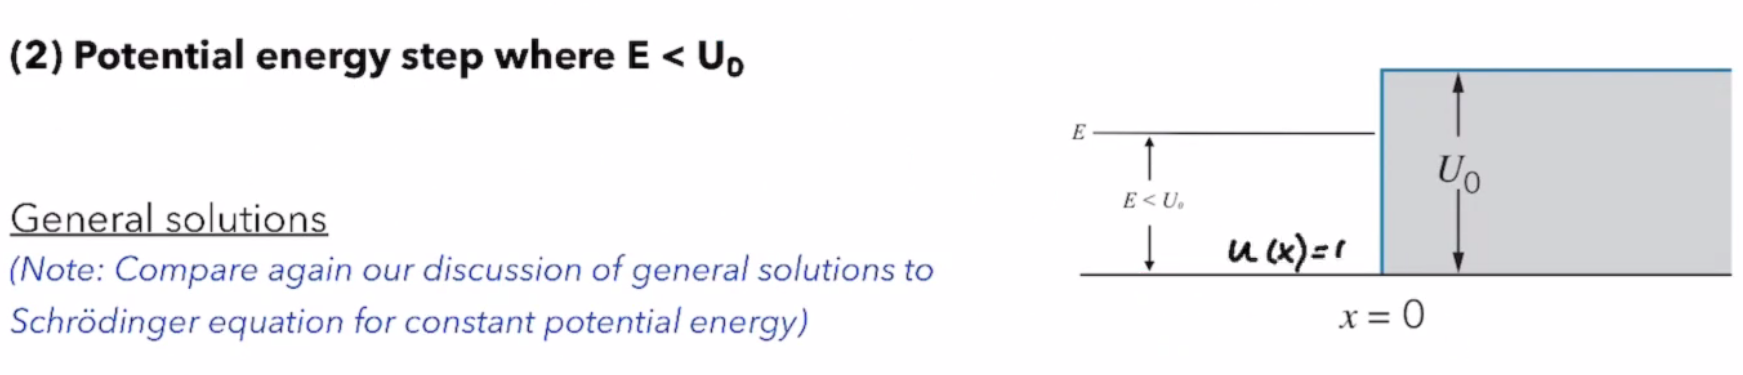
\includegraphics[width=1\linewidth]{./Images/pot_step2.png}
	\caption{}
\end{figure}

General solutions:
$$ For\ x<0: \psi_0(x) = A\ sin(k_0x) + B\ cos(k_0x)\ \ \ k_0 = \sqrt{\frac{2mE}{\bar{h}^2}} $$
$$ For\ x \geq 0:\ \Psi_1(x,t) = Ce^{k_1x} + De^{-ik_1x} \ \ \ k_1 =\sqrt{\frac{2m(U_0 - E)}{\bar{h}^2}} $$

As x approaches infinity, the C term approaches infinity, so it must be set to 0. \\

All particles are reflected from the barrier. We must have:
$$ x < 0:\ \Psi_0(x,t) = A'e^{i(k_0x-\omega t)} + B'e^{-i(k_0x+\omega t)} $$
With: $|A'|^2 = |B'|^2$

\subsubsection{Probability Density}
\begin{figure}[h!]
	\centering
	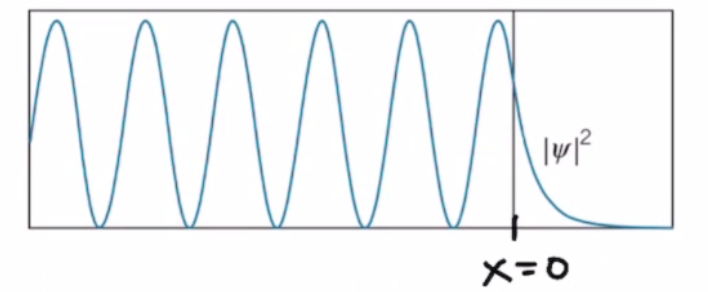
\includegraphics[width=0.6\linewidth]{./Images/pd_e_less_u.png}
	\caption{Probability Density (E $< U_0$). The region right of x=0 would be referred to the classically forbidden region. The probability density is nonzero.}
\end{figure}

\subsection{Energy Conservation \& Penetration into Forbidden Region}
Penetration into the forbidden region is associated with the wave nature of th eparticle as well as the uncertainty in the particle's energy or location (Heisenberg).\\

For probability density ($x > 0$):

$$ P(x) = |\psi(x)|^2 \propto |e^{-k_1x}|^2 = e^{-2k_1x} > 0 $$

To enter the forbidden region, the particle must temporarily gain energy to get over the potential energy step:

\begin{figure}[h!]
	\centering
	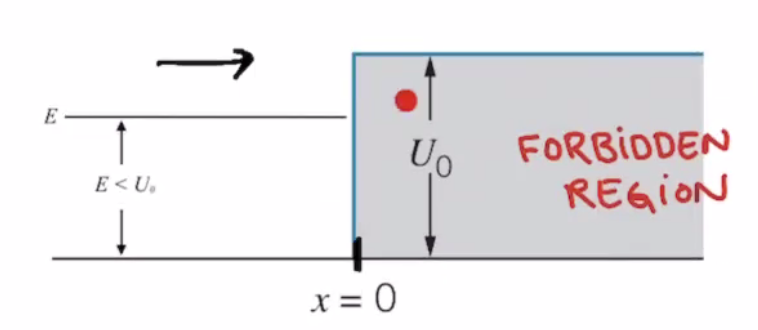
\includegraphics[width=0.6\linewidth]{./Images/forbidden_region.png}
	\caption{Must gain energy corresponding to ($U_0 - E$)}
\end{figure}

Supppose that the particle "borrows" energy sufficient to overcome the potential energy and gain a kinetic energy K:
$$ (U_0 - E) + K $$

This is OK according to Heisenberg's Uncertainty Principle!
$$ \Delta E \Delta t \geq \frac{\bar{h}}{2} $$

Because conservation of energy doesn't apply at times smaller than $\Delta t$ except within an amount:
$$ \Delta E \approx \frac{\bar{h}}{\Delta t} $$

\emph{Put another way, the particle can violate classical physics for a very short amount of time!} \\

From this, one can find the maximum penetration distance ($\Delta x_{max}$) into the forbidden region:

$$ \Delta x_{max} = \frac{\bar{h}}{1\sqrt{2m(U_0 - E)}} $$

\subsection{Potential Energy Barrier}
Next we consider a potential energy barrier:

\begin{figure}[h!]
	\centering
	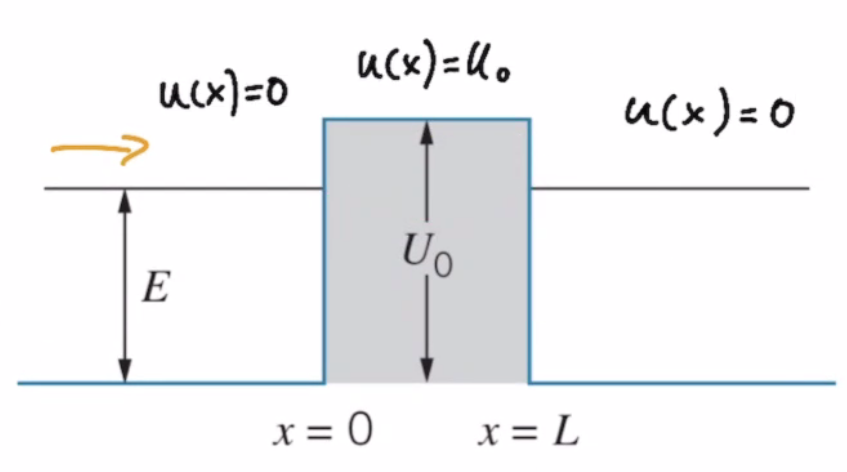
\includegraphics[width=0.6\linewidth]{./Images/potential_energy_barrier.png}
	\caption{Must gain energy corresponding to ($U_0 - E$)}
\end{figure}

Particles are incident from the left side of the barrier.

\begin{itemize}
	\item \textbf{Clasically}, we would never expect to find particles on the right side of the barrier ($x > L$), since their energy is insufficient to overcome the barrier.
	\item \textbf{Quantum Mechanically}, we do have particles transmitted!
\end{itemize}

This is known as quantum mechanical tunneling. Particles can never be observed in teh classically forbidden region, but they can ``tunnel" through it and be observed on the other side! \\

\emph{This is not a hypothetical but a REAL effect that can be observed}

\subsubsection{Analogy with Wave Optics}

If light passing through a glass prism reflects from an internal surface with an angle greater than the criticle angle, total internal reflection occurs.\\

However, the electromagnetic field actually decays exponentially just outside the prism. \\


\begin{figure}[h!]
	\centering
	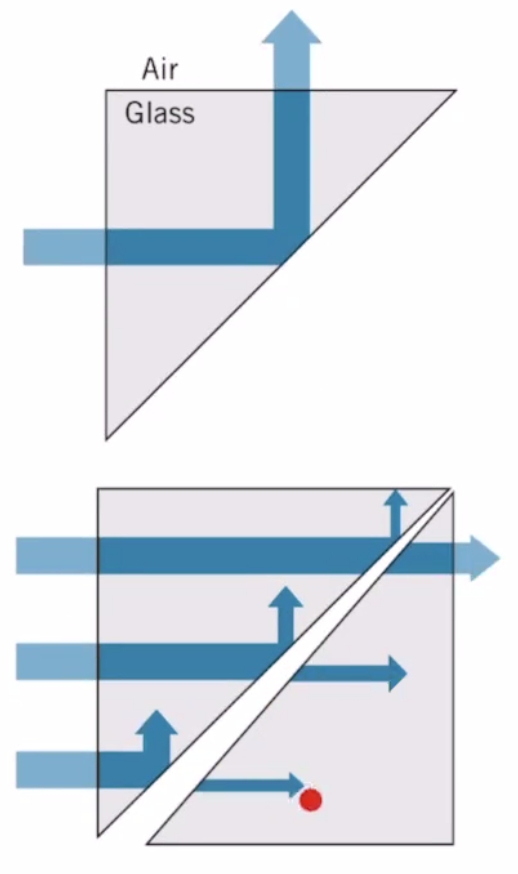
\includegraphics[width=0.2\linewidth]{./Images/prisms.png}
	\caption{}
\end{figure}

If we bring another prism very close to the first one, light passes into the second prism.\\

This is analgous to quantum-mechanical tunneling.

\newpage
\section{Practical Applications of Quantum Tunneling}
\subsection{Alpha decay}
Nuclei contain protons and neutrons, constantly moving. One type of radioactive decay is emittance of an alpha particle from the nuclei.\\
However, alpha particles must penetrate a potential energy barrier to escape the nucleus!\\
Measurements of this probability agree very well with quantum mechanical prediction.


\begin{figure}[h!]
	\centering
	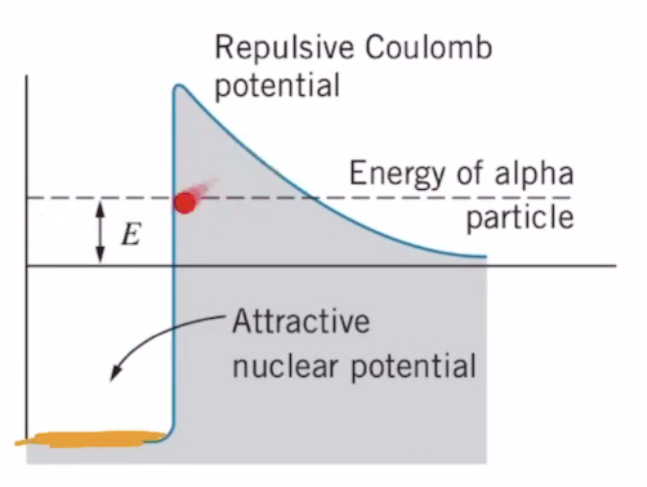
\includegraphics[width=0.6\linewidth]{./Images/alpha_tunneling.png}
	\caption{}
\end{figure}

\subsection{Scanning Tunneling Microscope}
Electrons trapped in a surface by a potential energy barrier (the work function of the material).\\
When a needle like probe is placed very close to the surface, electrons can tunnel through the barrier between surface \& probe - with a current that can be recorded.\\
This type of scanning tunneling microscope gives details corresponding to 1/100 of an atom.


\begin{figure}[h!]
	\centering
	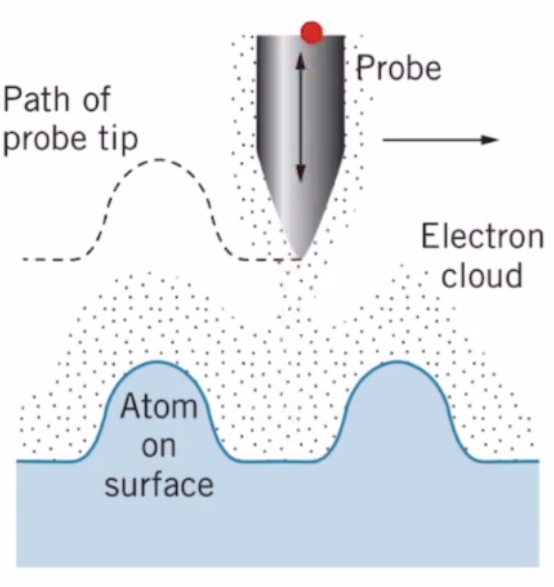
\includegraphics[width=0.6\linewidth]{./Images/tunneling_microscope.png}
	\caption{}
\end{figure}

\section{The Hydrogen Atom}
Ultimately, we must study the hydrogen atom in three dimensions. However, we'll start with just one dimension. \\
Note: When talking about a hydrogen atom, we assume no neutrons. \\
\begin{enumerate}
	\item Energy levels are the same as the Bohr's model
	\item Position of electron is NOT the same
		\begin{enumerate}
			\item Bohr's model gives fixed radii for the electron, where they revolve around the proton in a circular orbit.
			\item Quantum mechanics gives there's no ``fixed" radius or orbital plane, instead we must talk about probabilities
		\end{enumerate}
\end{enumerate}

Coulomb potential energy:
$$U(r) = -\frac{e^2}{4\pi\epsilon_0} * \frac{1}{r} $$

Schrödinger equation:
$$ -\frac{\bar{h}^2}{2m} \frac{d^2\psi}{dx^2}  - \frac{e^2}{4\pi\epsilon_0} * \frac{1}{x} \psi(x) = E\psi(x) $$

\newpage
The simplest wave function solution: \\
$ x > 0 $ \\
Bound state: $ \psi(x) \rightarrow 0\ when\ x \rightarrow \infty $ \\

$$ \psi(x) = A xe^{-bx} $$

If we substitute into the Schrödinger equation:
$$ b = \frac{me^2}{4\pi\epsilon_o\bar{h}^2} \leftarrow\ This: \ = \frac{1}{a_0} $$
$a_0 = 0.0529$

Corresponding energy is identical to energy of ground state in the Bohr model!\\


\begin{figure}[h!]
	\centering
	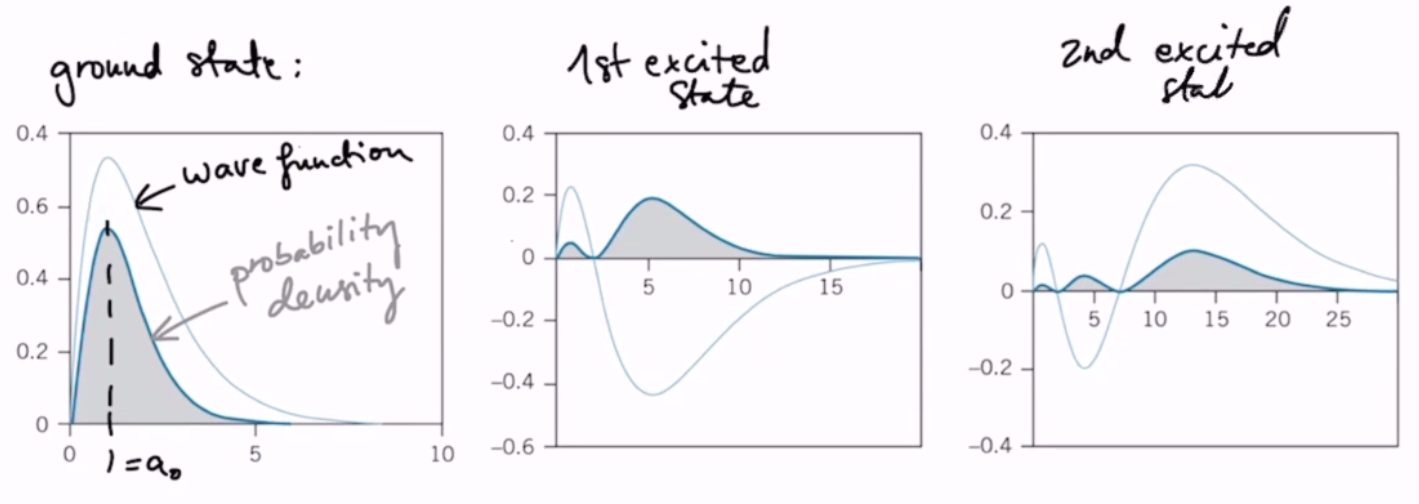
\includegraphics[width=0.9\linewidth]{./Images/probability_electrons.png}
	\caption{Simplified 1-dimensional version}
\end{figure}

\newpage
\begin{question}[Example]
	What is the normalization constant for the ground-state wave function for the one-dimensional Coulomb potential?
	$$ \psi(x) = Axe^{-bx},\ b = \frac{1}{a_0},\  A = ? $$
	\begin{answer}[Answer]
		$$ 1 = \int_0^\infty |\psi(x)|^2\ dx = \int_0^\infty |Axe^{-\x/a_0} |^2\ dx $$
		$$ = A^2 \int_0^\intfy x^2 e^{-2x/a_0} dx $$
		$$ \int_0^\infty x^n e^{-cx} dx = \frac{n!}{c^{n+1}} $$
		$ n = 2,\ c = \2/a_0 $ \\
		$$ 1 = A^2 \frac{2!}{(2/a_0)^3} = A^2 \frac{2a_0^3}{2^3} $$
		Solve for A:
		$$ A = \sqrt{\frac{2^3}{a_0^3}} = (2a_0)^{-3/2} $$
	\end{answer}
\end{question}

\subsection{Angular Momentum and the Hydrogen Atom (and you!)}
Remember: Bohr model used the idea that angular momentum was quantized \\

\textbf{Classical orbits} \\
Angular momentum of a particle:
$$ \vec{L} = \vec{r} \times \vec{p} $$

where: \\
$ \vec{L} $: angular momentum vector \\
$ \vec{r} $: position vector \\
$ \vec{p} $: linear momentum vector \\


\begin{figure}[h!]
	\centering
	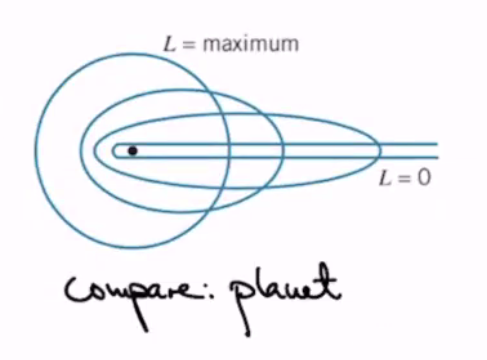
\includegraphics[width=0.5\linewidth]{./Images/angular.png}
	\caption{Angular momentum remains constant}
\end{figure}

\subsection{Angular Momentum in Quantum Mechanics}

Angular momentum in quantum mechanics looks a bit different...\
For a three-dimensional wave function there are two associated quantum numbers:

\begin{itemize}
	\item Angular momentum quantum number ($l$) determines length of angular momentum vector ($\vec{L}$):
		$$ |\vec{L}| = \sqrt{l(l+1)} \bar{h} \ \ \ l=0,1,2,....$$
		\emph{Borh said $|\vec{L}| = n \bar{h}$|}
	\item Magnetic quantum number ($m_l$) tells us about the z-component of the angular momentum vector:
		$$ L_z = m_l \bar{h} \ \ \ m_l = 0, +-1, +-2, ... +- l $$
\end{itemize}

\begin{question}[Example]
	Compare the length and z-component of angular momentum vector that represents the orbital motion of an electron in quantum states: $l = 1\ vs\ l=2$
	$l = 1$:
	$$ |\vec{L}| = \sqrt{l(l+1)}\bar{h} = \frac{2}\bar{h} $$
	$m_l\ if\ l=1?\ \ \ m_l = 0, +- 1$ \\
	$L_z = m_l \bar{h}$, possible values: $L_z = -\bar{h}, 0, \bar{h}$
	$l = 2$:
	$$ |\vec{L}| = \sqrt{l(l+1)}\bar{h} = \frac{6}\bar{h} $$
	$m_l\ if\ l=2?\ \ \ m_l = 0, +- 1, +- 2$ \\
	$L_z = m_l \bar{h}$, possible values: $L_z = -2\bar{h}-\bar{h}, 0, \bar{h}, 2\bar{h}$

	Polar angle $\theta$ that vector L makes with z-axis:
	$$ cos(\theta) = \frac{L_z}{|\vec{L}|} = \frac{m_l}{\sqrt{l(l+1)}} $$

\end{question}

\begin{figure}[h!]
	\centering
	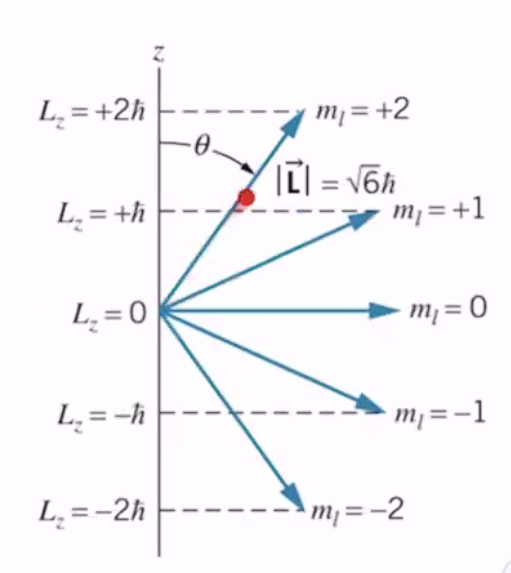
\includegraphics[width=0.2\linewidth]{./Images/l_equals_2.png}
	\caption{Graphical representation for the l=2 scenario}
\end{figure}

``Spacial quantization" - only certain orientations of angular momentum vectors are allowed. Number of allowed orientations? 2L + 1

\subsection{The Angular Momentum Uncertainty Relationships}

\begin{itemize}
	\item In quantum mechanics, the maximum information known about the angular momentum vector is the length and z-component.
	\item To fully describe a three-dimensional vector requires three numbers....
	\item There is an uncertainty (indeterminacy) in specifying the angular momentum vector
\end{itemize}

$$ \Delta L_z \Delta \phi \geq \bar{h} $$

\begin{figure}[h!]
	\centering
	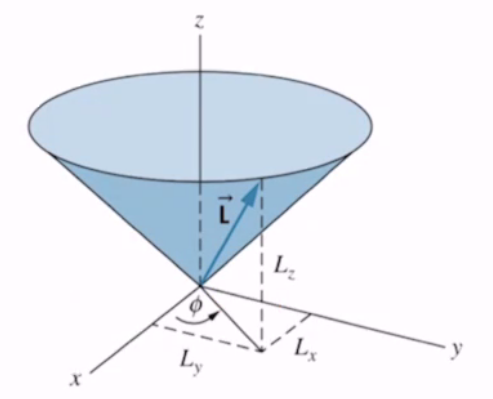
\includegraphics[width=0.3\linewidth]{./Images/angular_2.png}
	\caption{We don't have enough components to determine all dimensions - thus we need $phi$ to find the angle}
\end{figure}

\emph{When one component of $L_x, L_y, L_z$ is determined, we known nothing about the other two.}

\subsubsection{Spherical Polar Coordinates}

\begin{figure}[h!]
	\centering
	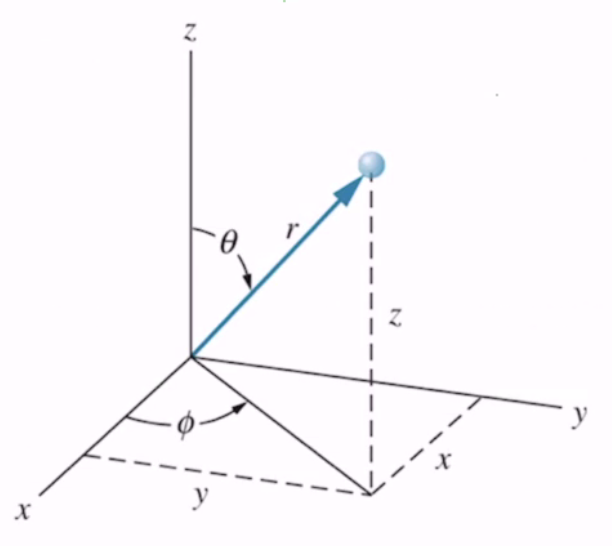
\includegraphics[width=0.5\linewidth]{./Images/spherical_coordinates.png}
	\caption{$x = rsin\theta\ cos\phi$, $y = rsin\theta\ sin\phi$, $z = rcos\theta$}
\end{figure}

$$ x^2 + y^2 + z^2 = r^2 $$
$$ cos\theta = \frac{z}{r} $$
$$ tan\phi = \frac{y}{x} $$


\subsection{Schrödinger Equation in Three Dimensions}
In Cartesian coordinates:
$$ -\frac{\bar{h}^2}{2m} \left(\frac{\delta^2\psi}{\delta x^2} + \frac{\delta^2\psi}{\delta y^2} + \frac{\delta^2\psi}{\delta z^2} \right) + U(x, y, z) \psi(x, y, z) = E \psi(x, y, z) $$ 

\begin{figure}[h!]
	\centering
	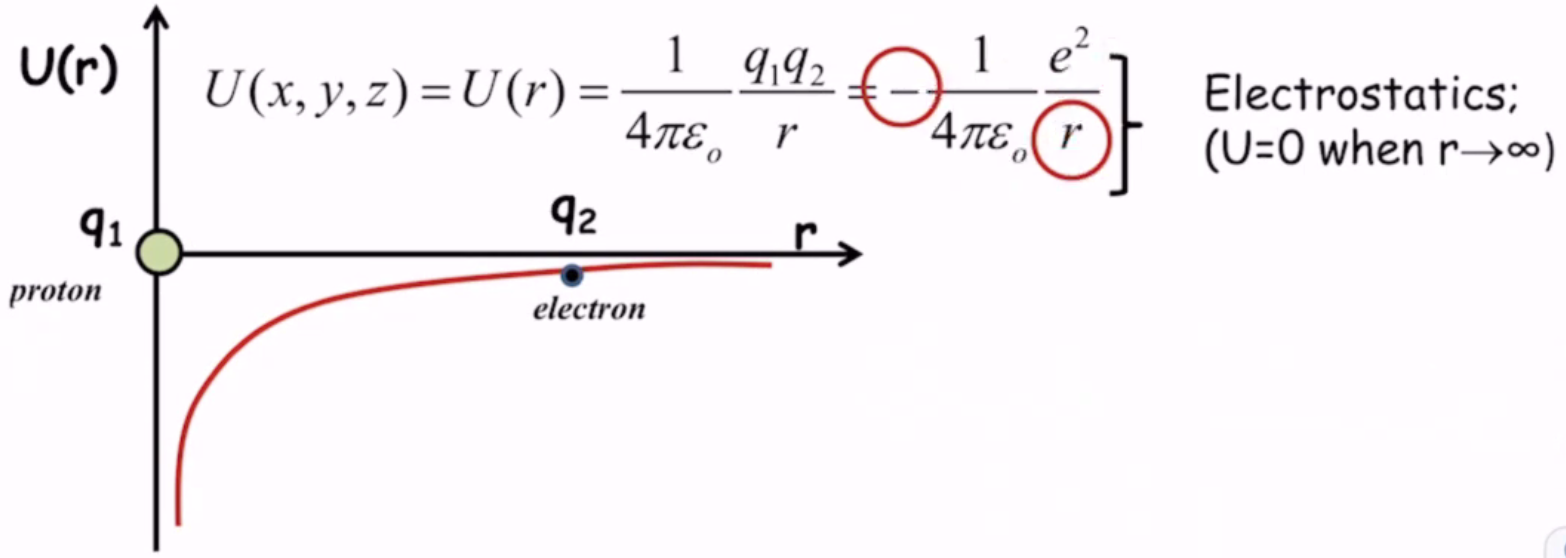
\includegraphics[width=.8\linewidth]{./Images/electrostatics.png}
	\caption{This would get very messy if we tried to solve it}
\end{figure}

It's more convenient to work in spherical coordinates ($r, \theta, \phi$) to obtain a separable solution:
$$\psi(r, \theta, \phi) = R(r) \Theta(\theta) \Phi(\phi) $$
Radial function, polar function, azimuthal function. \\

Reminder -- spherical polar coordinates:\\
$ x = rsin(\theta) cos(\phi) $ \\
$ y = rsin(\theta) sin(\phi) $ \\
$ z = rcos(\theta) $ \\

Our pentalty for this change of coordinates is a more complex Schrödinger equation:

$$ -\frac{\bar{h}^2}{2m} \left(\frac{\delta^2\phi}{\delta r^2} + \frac{2}{r}\frac{\delta \phi}{\delta r} + \frac{1}{r^2 sin(\theta)} \frac{\delta}{\delta \theta} \left(sin\theta \frac{\delta\phi}{\delta \theta} \right) + \left(sin^2\theta \frac{\delta^2\phi}{\delta \phi^2} \right) \right) + U(r, \theta, \phi) \psi(r, \theta, \phi) = E\psi(r, \theta, \phi) $$
Hydrogen the U function is just U(r).

With our separabel function written as above, this allows us to split the equation into three separate differential equations:

\begin{itemize}
	\item Azimuthal: 
		$$ \frac{d^2\Phi}{d\phi^2} + m_2^2 \Phi(\phi) = 0 $$
	\item Polar: 
		$$ \frac{1}{sin\theta} \frac{d}{d\theta} \left( sin\theta \frac{d\Theta}{d\theta} \right) + \left( l(l+1) - \frac{m_l^2}{sin^2\theta} \right) \Theta(\theta) = 0 $$
	\item Radial:
		$$ -\frac{\bar{h}}{2m} \left( \frac{d^2R}{dr^2} + \frac{2}{r} \frac{dR}{dr} \right) + \left( \frac{-e^2}{4 \pi \epsilon_o r} + \frac{l(l+1) \bar{h}^2}{2mr^2} \right) R(r) = E R(r) $$
\end{itemize}
Where: \\
m: electron mass \\
($r, \theta, \phi$): electron position in polar coordinates \\
E: Total energy \\
and some quantum numbers.


\subsubsection{More on these Quantum Numbers}
When we solved the one-dimensional Schrödinger equation for the infinite potential energy well, we found that our solutions for allowed wavelength and energies were quantized. The index, or quantum number, ``n" appeared  in our solutions. \\

Similarly when solving the three-dimensional Schrödinger equation, \textbf{three} parameters emerge as indices. Only certain values for these are allowed to ensure that solutions are physical and don't diverge. These are \emph{three quantum numbers} that describe the solutions:
\begin{itemize}
	\item Principle quantum number: n of n = 1,2,3 fame
	\item $l$ where (l = 0, 1, 2, 3,.. n-1)
	\item $m_l$ where ($m_l$ = 0, +-1, +-2, ... +- $l$) 
\end{itemize}
Same as discussed yesterday!


\begin{result}[Quantized Energy Levels]
	$$ E_n = -\frac{me^4}{32\pi^2\epsilon_0^2\bar{h}^2} = \frac{-13.60\ eV}{n^2} $$
	Same as in the Bohr's model, sweet \\
\end{result}

\begin{result}[Wave Function Solutions]
	$$ \psi_{n, l, m_l}(r, \theta, \phi) = R_{n,l}(r) \Theta_{l, m_l} \Phi_{m_l}(\phi) $$
\end{result}

\subsubsection{Degeneracy}
Different sets of quantum numbers can correspond to exactly the same energy. This is known as ``degeneracy", and such an energy level is said to be ``degenerate". \\

Ground state of hydrogen atom:
$$ E_n = \frac{-13.60\ eV}{n^2} \rightarrow n = 1: \rightarrow E_1 = -13.60\ eV $$
$n, l, m_l: 1, 0, 0$

First excited state:\\
n = 2:
$$ E_2 = \frac{-13.60\ eV}{2^2} = -3.40\ eV $$
$[n, l, m_l]: [2, 0, 0],[2, 1, 0],[2, 1, -1], [2, 1, 1] $ \\
\emph{Generally: State n $\rightarrow n^2$ degenerate} \\

Why do we still list these separately?
\begin{enumerate}
	\item Levels are not precisely degenerate (1 e-5 eV separations)
	\item We will see that transitions between energy levels depend on quantum numbers of energy level that transition starts from
	\item Each set of quantum numbers correspond to a different \emph{wave function}, and thus a different \emph{state of motion} for an electron (different probability densities)
\end{enumerate}

\subsection{Probability Densities}
Probability density for one-dimensional wave function: $P(x) = |\psi(x)|^2$ \\
Note: wave function can be complex, so this is wave function times its complex conjugate $ |\psi|^2 = \psi\psi*$ \\

We are now working in THREE dimensions, so we need volume probability density:

$$P(r, \theta, \phi) = |\psi(r, \theta, \phi)|^2 $$

Probability to find electron in a small volume centered at ($r, \theta, \phi$) is:

$$P(r, \theta, \phi) dV \ \ (volume\ element) $$
In cartesian coordinates $dV: dxdydz$. But, in polar:
$$ dV = r^2 sin\theta dr d\theta d\phi $$


\begin{figure}[h!]
	\centering
	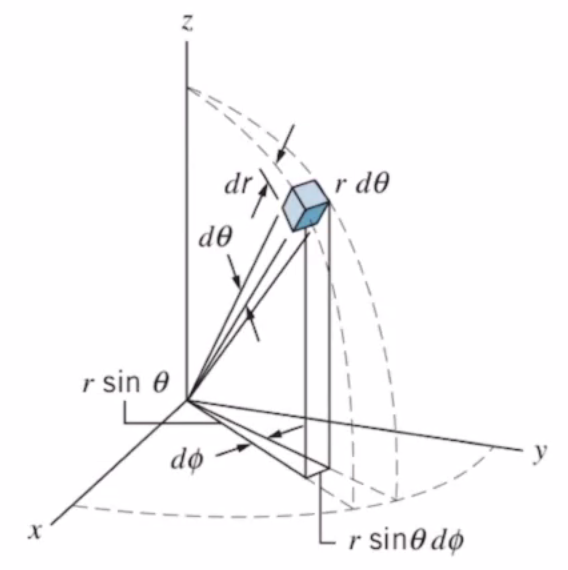
\includegraphics[width=.3\linewidth]{./Images/3d_probability.png}
	\caption{Finding the probability of finding the electron in some tiny volume element}
\end{figure}

Or, written out in terms of the separable wave function:
$$ |\psi(r, \theta, \phi)|^2 dV = |R_{n,l}(r)|^2 |\Theta_{l,m_l}(\theta)|^2 |\Phi_{m_l}(\phi)|^2 r^2 sin\theta dr\ d\theta\ d\phi $$

We can think of these as smeared out distributions of electric charge in the atom, due to uncertainty in locating the electron. Or, the statistical result of large numbers of measurements of the electron's position.\\


\begin{figure}[h!]
	\centering
	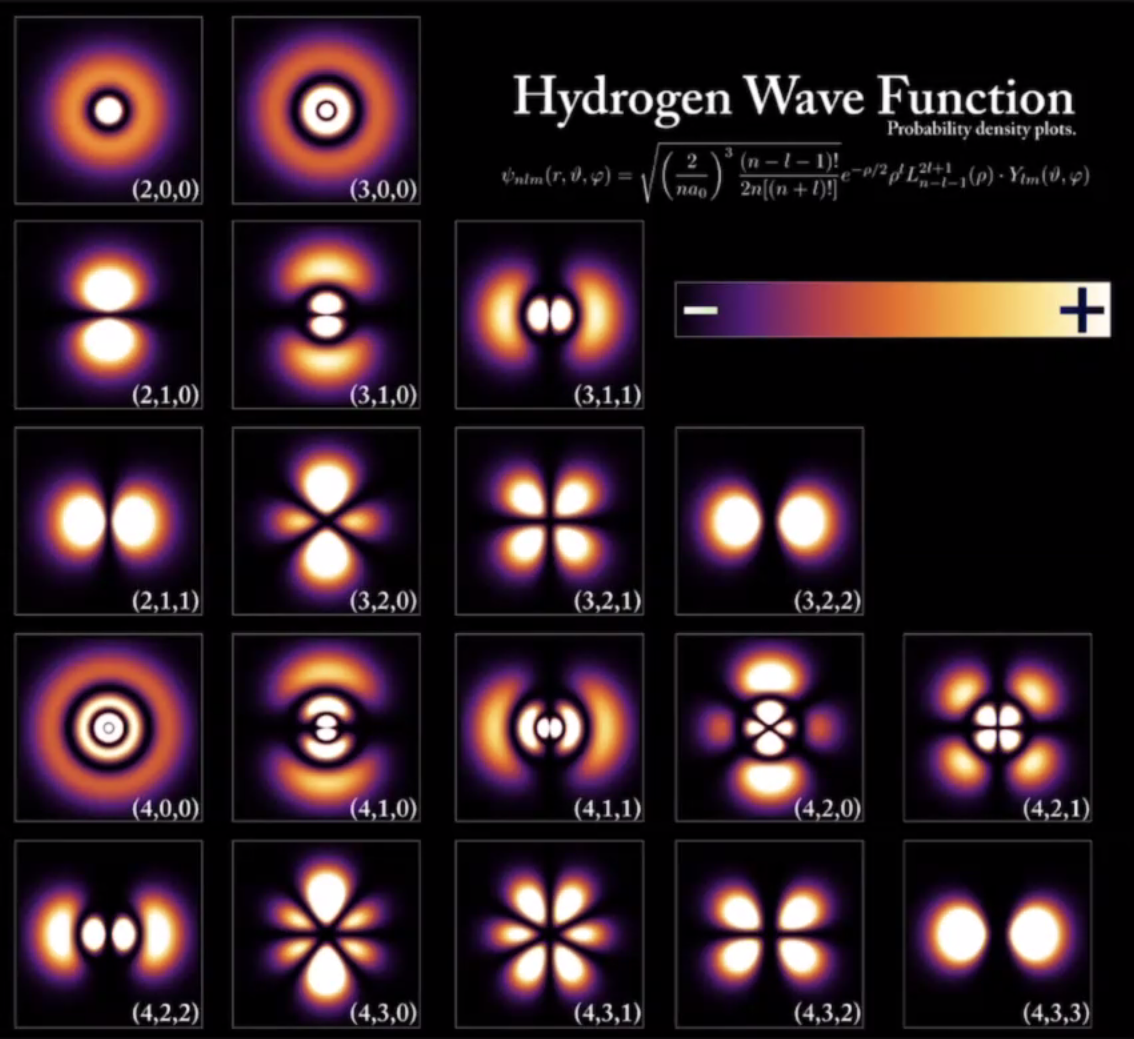
\includegraphics[width=1\linewidth]{./Images/hydrogen_wave_function.png}
	\caption{Finding the probability of finding the electron in some tiny volume element}
\end{figure}

\newpage
\subsubsection{Radial Probability Density}
Consider just the probability to locate the electron at a particular radial distance from the nucleus. You can just integrate over the $\theta, \phi$ coordiates!:

$$ P(r) dr = |R_{n,l}(r)|^2 r^2\ dr \ \int_0^\pi |\Theta_{l, m_l}(\theta)|^2 sin\theta\ d\theta\ \int_0^{2\pi} |\Phi{m_l}(\phi)|^2 d\phi $$ 
But hey, if you integrate over all valid values of the angular components, they just end up being 1 because the wave function is normalized! So we get:

$$ P(r) = $r^2 |R_{n, l}(r)|^2 $$


\begin{figure}[h!]
	\centering
	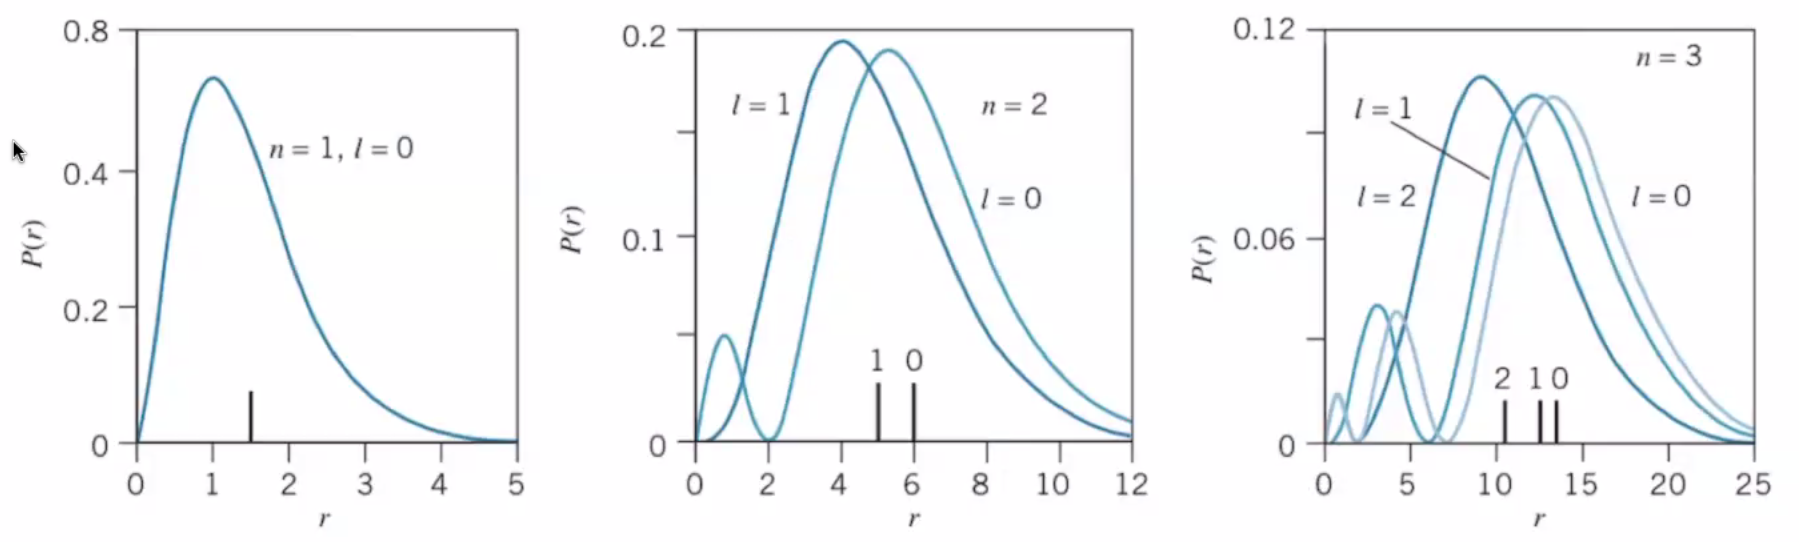
\includegraphics[width=1\linewidth]{./Images/radial_probability_densities.png}
	\caption{The probability density of r alone. The highest point won't necessarily line up with the radius predicted by Bohr? The lower you go for l the more little peaks you get.}
\end{figure}

\subsubsection{Angular Probability Density}

Consider instead the angular probability density:
$$ P(\theta, \phi) = |\Theta_{l, m_l}(\theta)\Phi_{m_l}(\phi)|^2 $$
Note: These are all cylindrically symmetric.


\begin{figure}[h!]
	\centering
	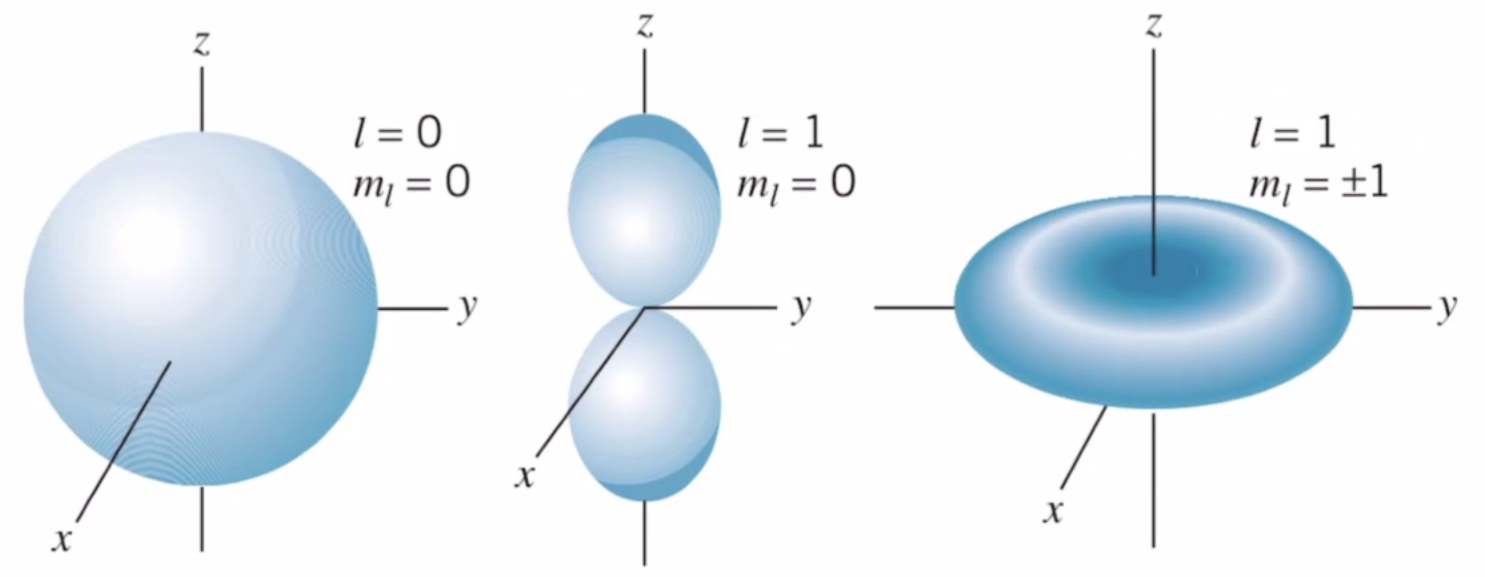
\includegraphics[width=1\linewidth]{./Images/cylindric.png}
	\caption{}
\end{figure}


\subsection{Time-Dependence}
We are working with stationary states which won't change with time.
$$ I\ missed\ this $$

\newpage
\begin{question}[Example]
	For the n=2 states (l=0, l=1), compare the radial probabilities of finding the electron inside the Bohr radius?

	$$ R_{2,0}(r) = \frac{1}{(2a_0)^{3/2}} \left(2 - \frac{r}{a_0} \right) e^{-r/2a_0} $$

	Radial Probability:
	$$ P(r) dr = r^2 |R_{n,l}(r)|^2\ dr \ \ \ \ \ 0 \leq r < a_0 $$

	for n=2, l=0:
	$$ P(0:a_0) = \int_0^a_0 P(r) dr = \int_0^a_0 r2 \frac{1}{(2a_0)^{3}} \left(2 - \frac{r}{a_0} \right)^2 e^{-r/a_0}  dr  $$
	$$ = \frac{1}{8a_0^3} \int_0^a_0 \left(4r^2 - \frac{4r^3}{a_0} + \frac{r^4}{a_^2} \right) e^{-r/a_0}\ dr $$

	To solve these types of integrals:
	$$ \int x^n e^{-cx} dx = - \frac{e^{-cx}}{c} \left( x^n + \frac{nx^{n-1}}{c} + \frac{n(n-1)x^{n-2}}{c^2} ... + \frac{n!}{c^n} \right) $$

	$$ P(0:a_0) = 0.034 $$

	If we do the same for the n=2, l=1 state:
	$$ P(0:a_0) = 0.0037 $$
\end{question}

\subsection{Magnetic Moments}
The orbital angular momentum of the electron is related to its magnetic dipole moment.
\begin{figure}[h!]
	\centering
	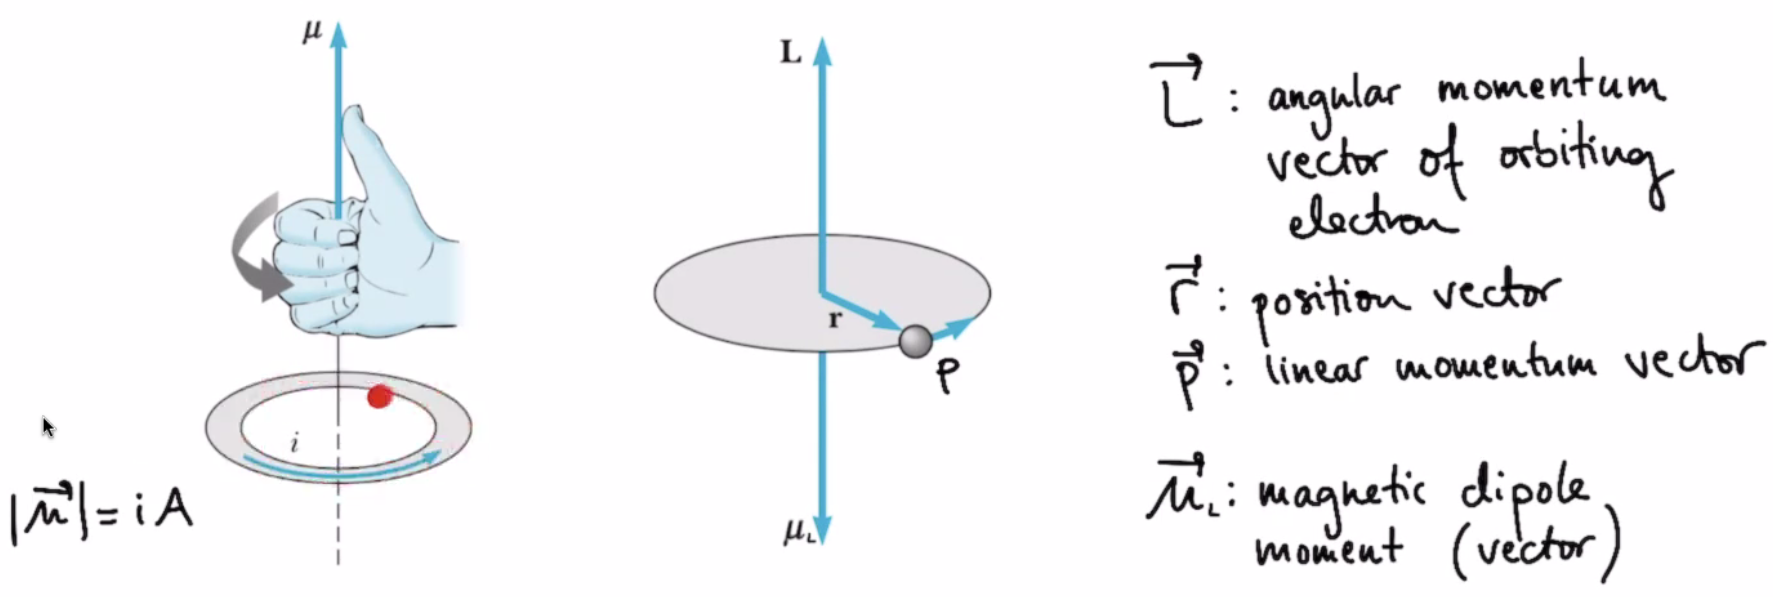
\includegraphics[width=1\linewidth]{./Images/magnetic_moment.png}
	\caption{The direction of current is by convention that of positive charge, while the electron is negatively charged. Note the subscript ``L" on $\vec{u}$}
\end{figure}
Electron's orbital magnetic dipole moment (follows from considering orbiting electron as a circular loop of current):
$$ \vec{u_L} = -\frac{e}{2m} \vec{L} $$

The z-component of the magnetic moment:
$$ \vec{\mu_{L_z}} = -\frac{e}{2m} L_z = -\frac{e}{2m} m_l \bar{h} $$
Where $m_l$ is the magnetic quantum number and m is the electron mass.

Bohr magneton defined as:
$$ \mu_B = \frac{e\bar{h}}{2m} \approx 9.274 \cdot 10^{-24} J/T \rightarrow \mu_L_z = -m_l \mu_B $$

\textbf{What happens to a magnetic dipole moment ($\vec{\mu}$) in an external magnetic field ($\vec{B}$)? }\\
It experiences a torque:
$$ \vec{\tau} = \vec{\mu} \times \vec{B} $$
Analagous to an electric dipole moment in an external electric field:



\begin{figure}[h!]
	\centering
	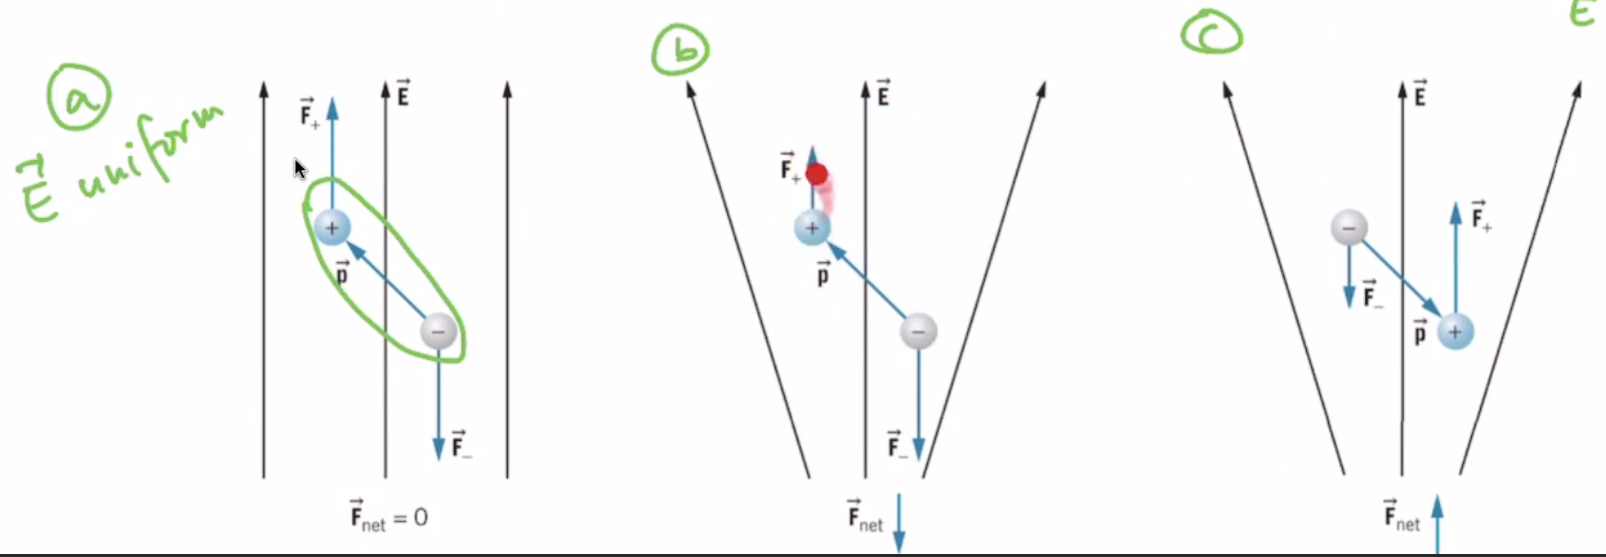
\includegraphics[width=1\linewidth]{./Images/electric_dipole.png}
	\caption{B + C non-uniform E-field.}
\end{figure}


\begin{figure}[h!]
	\centering
	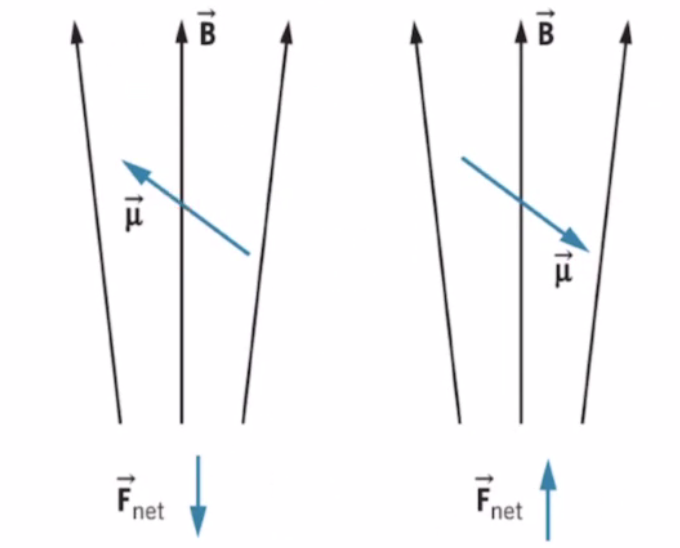
\includegraphics[width=.6\linewidth]{./Images/magnetic_dipole.png}
	\caption{Magnetic dipoles in nonuniform magnetic field experience a net force (direction depending on direction dipole is pointing in)}
\end{figure}

\newpage
\textbf{What should happen to atoms passing through a region of nonuniform magtnetic field?}\\
For hydrogen: $\mu_{L,z} = -m_l \mu_B$ \\
if $n=1, l = 0 \rightarrow m_l = 0 \rightarrow \mu_{Lz} = 0 \rightarrow$ no deflection\\
if $n=2, l = 1 \rightarrow m_l = 0, \pm 1 \rightarrow \mu_{Lz} = 0, \pm \mu_{b} $ \\

\subsubsection{Stern-Gerlach Experiment}
Initially done in 1921 using silver atoms -- more complicated structure than hydrogen atom but same general principle. Repeated in 1927 using hydrogen atoms.

\begin{figure}[h!]
	\centering
	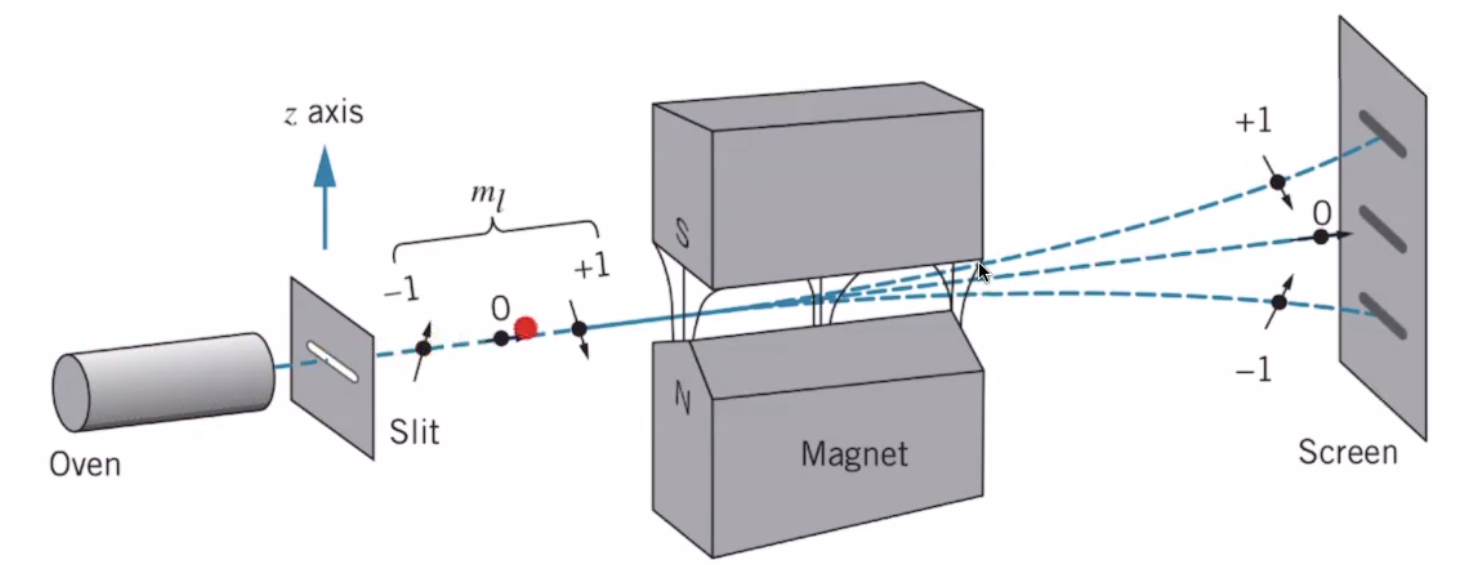
\includegraphics[width=1\linewidth]{./Images/gerlach.png}
	\caption{n=2, l=1, $m_l$ = -1, 0, +1. Expectation was that the beam will be split in (2l + 1), the number of quantum numbers.}
\end{figure}

\textbf{Experimental result}: Beams were split in \textbf{TWO}?!? \\
$ 2 \cdot S + 1 = 2 \cdot 1/2 + 1 = 2 $ \\

\begin{figure}[h!]
	\centering
	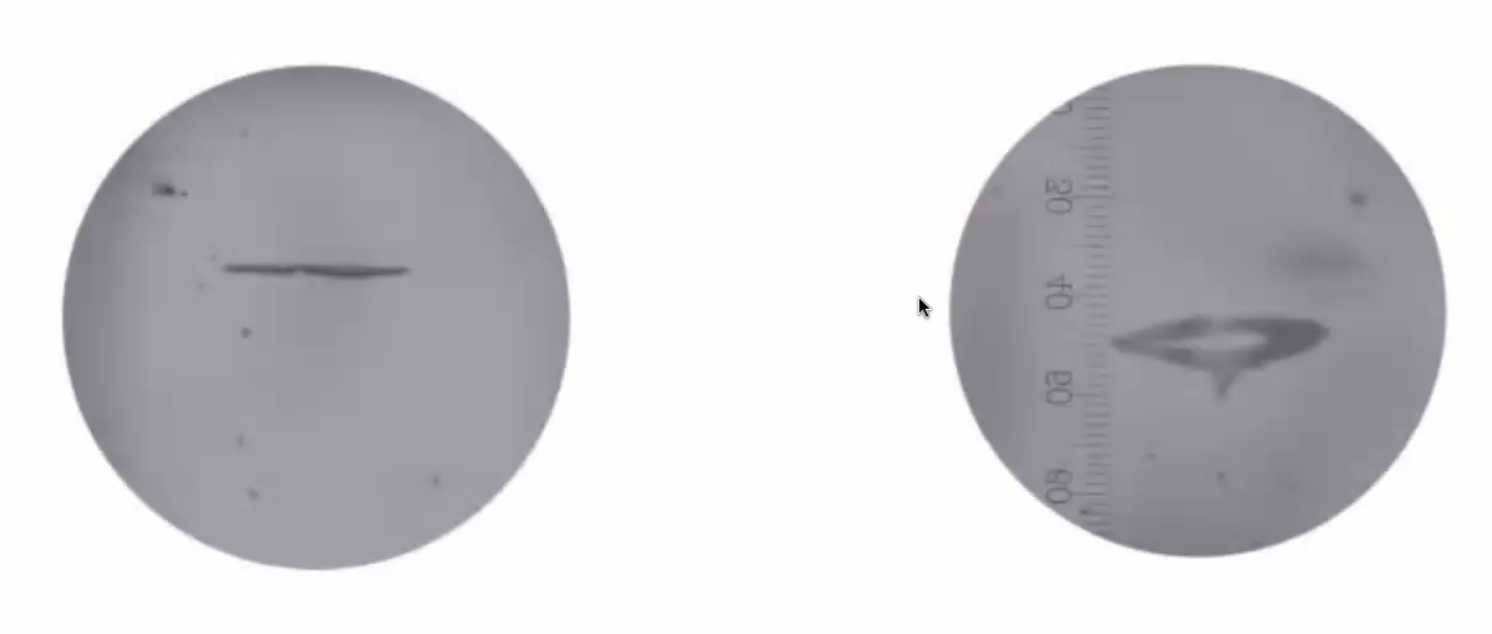
\includegraphics[width=.8\linewidth]{./Images/gerlach_results.png}
	\caption{Left: Magnetic field OFF. Right: Magnetic field ON}
\end{figure}

Explanation:
There is an additional component to the electron's angular momentum, with an associated magnetic moment. This turns out to be an intrinsic property of the electron (like its mass or charge), called intrinsic \textbf{\emph{spin}}.\\

An electron has an \textbf{intrinsic spin quantum number s = 1/2} (it has ``spin 1/2"). \\

\emph{Spin is a property of all elementary particles: photon has ``spin 1", Higgs boson has a ``spin 0".} \\

\subsection{Intrinsic Spin}

Spin ends up being super important when dealing with multiple electrons. \\

\begin{itemize}
	\item Electron has orbital angular momentum: $ \vec{L} $
	\item Electron has intrinsic angular momentum: $ \vec{S} $
\end{itemize}

\begin{figure}[h!]
	\centering
	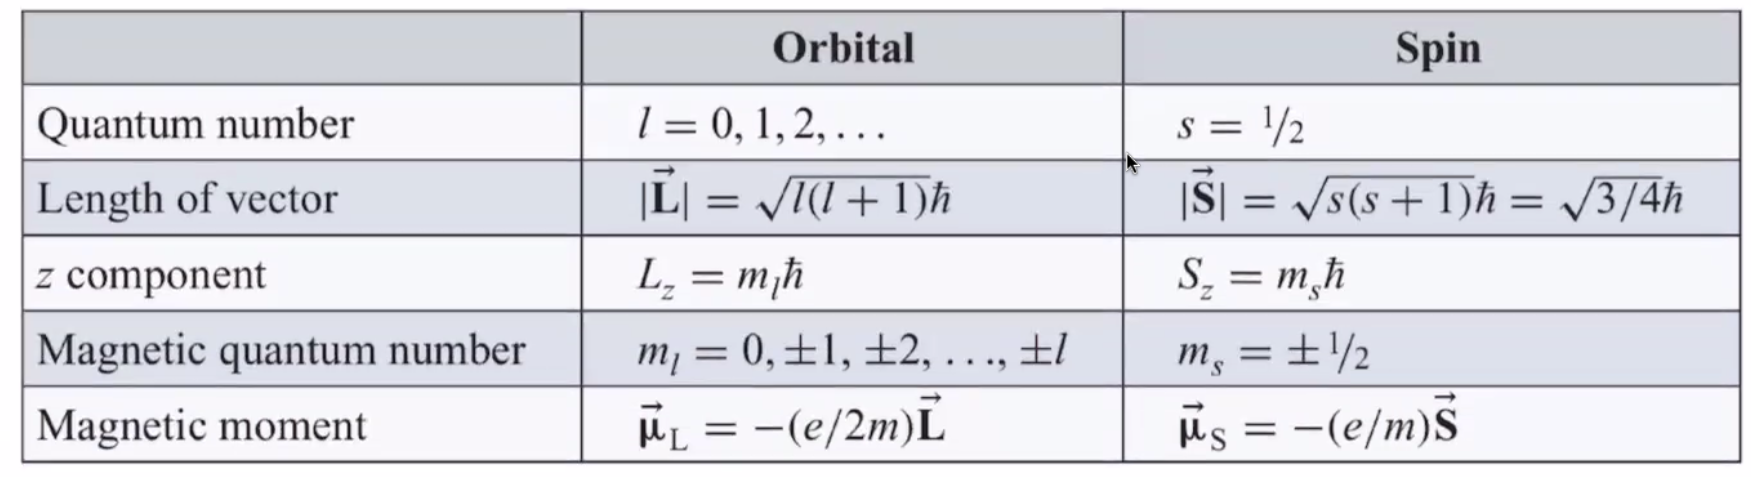
\includegraphics[width=1\linewidth]{./Images/spin.png}
	\caption{These are very very similar.}
\end{figure}


\begin{figure}[h!]
	\centering
	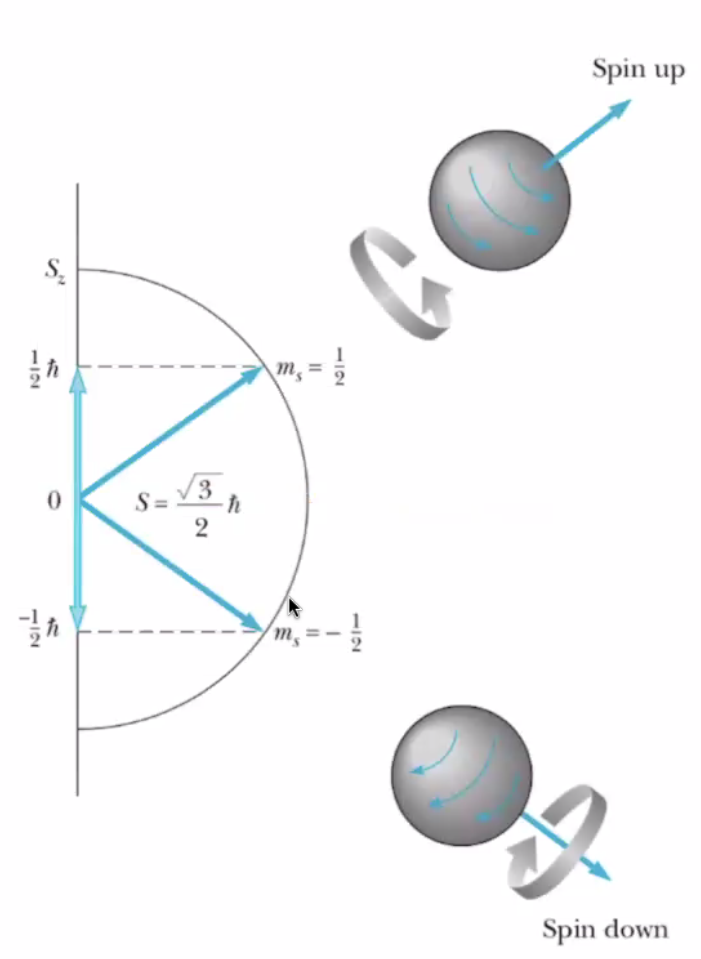
\includegraphics[width=.45\linewidth]{./Images/spin_up.png}
	\caption{We talk about ``spin up" vs ``spin down". Note: While thinking about intrinsic spin as the electron spinning about its own axis, in the same way as the Earth spins about its own axis -- ``spin angular momentum" + orbits about the sun ``orbital angular momentum" is a useful image, but it is physically incorrect as the electron is a point particle with no physics size.}
\end{figure}

\subsubsection{Energy Levels (Reloaded)}
We in fact need to use FOUR quantum numbers to fully describe the electronic states in hydrogen:
$$ n, l, m_l, m_s \ \ \ (s = 1/2\ for\ electrons)$$

Degeneracy of a given energy level ``n" is: $ 2n^2 $ \\

Usually it is sufficient to specify (n, l) for these energy levels: \textbf{spectroscopic notation:}

\begin{figure}[h!]
	\centering
	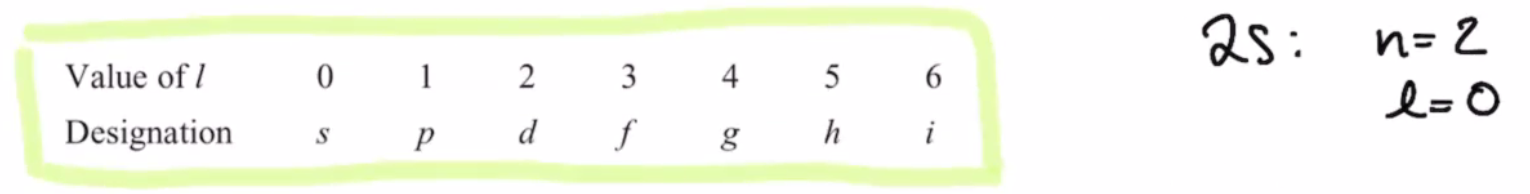
\includegraphics[width=.45\linewidth]{./Images/spectroscopic.png}
	\caption{}
\end{figure}

\subsubsection{Fine Structure (bonus)}
We are now equipped to discus why energy levels are not really 100\% degenerate as mentioned yesterday... this is called ``find structure".\\

From electron's perspective, it is being orbited by a positively charged proton. This ``proton current" causes a magnetic field at the electron, which interacts with the electron's spin magnetic moment. This results in a small energy difference between ``spin up" and ``spin down" states: \\

$$ \Delta E = 2 \mu_B B $$
For the bohr magneton and effective induced magnetic field. \\
\begin{figure}[h!]
	\centering
	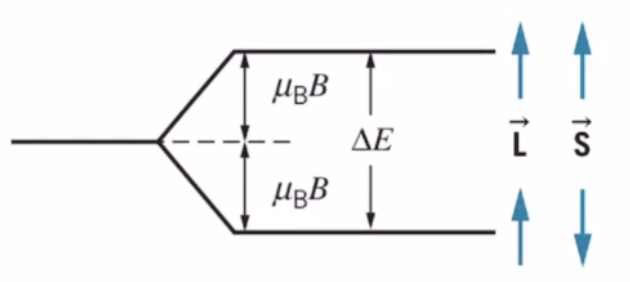
\includegraphics[width=.25\linewidth]{./Images/non-degeneracy.png}
	\caption{}
\end{figure}
To fully determine this quantitatively, one must consider relativistic quantum mechanics (way beyond the scope of this course). But the difference is on the order of 0.00001 eV.


\subsection{Probability, again?}

\begin{question}[Example]
	From the n=2, l=1, $m_l = 0$ wave function, find the directions in space at which the maximum probability occurs.

	\begin{answer}[Answer]
		$$ P(\theta, \phi) = |\Theta_{l, 0}(\theta) \Phi_0(\phi)|^2 $$
		$$ = | \sqrt{\frac{3}{2}} cos \theta \cdot \frac{1}{\sqrt{2\pi}} |^2 = \frac{3}{4\pi}cos^2\theta $$
		Note that there is no dependence on phi. \\
		Maximum probabiliy?
		$$\frac{dP}{d\theta} = \frac{3}{4\pi}(-2 cos\theta \cdot sin \theta) = 0 $$
		$$ =  cos\theta = 0 \rightarrow \theta = \frac{\pi}{2} $$
		$$ =  sin\theta = 0 \rightarrow \theta = 0, \pi $$

		Max or min?
		$$ \frac{d^2P}{d\theta^2} = \frac{3}{2\pi} (sin^2\theta - cos^2\theta) $$
		if $\theta = \pi/2$, second derivative is greater than zero, so it's a minimum.
		if $\theta = 0, \pi$, second derivative is less than zero, so it's a maxiumu.
	\end{answer}
\end{question}

\section{Many-Electron Atoms}
\begin{itemize}
	\item When we begin to consider atoms with more than one electron, potential energy now depends both on:
	\begin{itemize}
		\item An attractive Coulomb potential between the electrons and nucleus
		\item A repulsive Coulomb potential between different electrons
	\end{itemize}
	\item We quickly fail to solve exactly the Schrödinger's equation
	\item Instead, solutions are obtained numerically
\end{itemize}

\subsection{Pauli's Exclusion Principle}
We have seen that an atomic electron is described by four quantum numbers:
$$ n, l, m_l, m_s\ where\ s = 1/2\ always\ for\ electrons $$
How many electrons in an atom can have the same four quantum numbers? I.e. how many electrons in an atom can be in the same state?
\begin{figure}[h!]
	\centering
	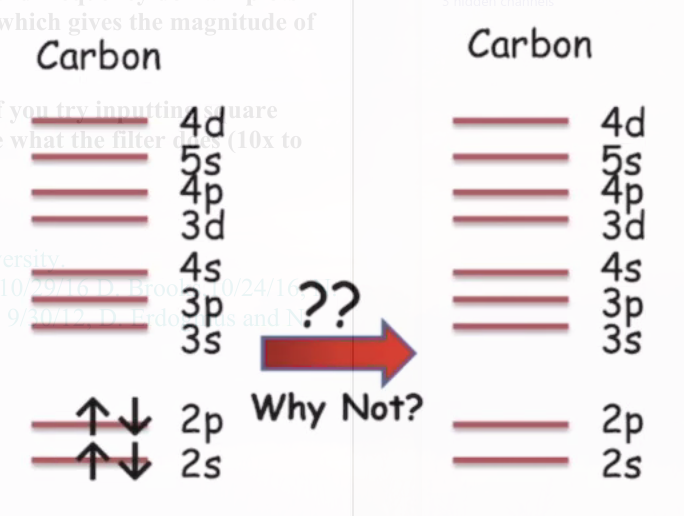
\includegraphics[width=.25\linewidth]{./Images/carbon_electrons.png}
	\caption{}
\end{figure}

\begin{result}[Pauli's exclusion principle]
	No two electrons in an atom can have the same set of quantum numbers!
\end{result}

\begin{figure}[h!]
	\centering
	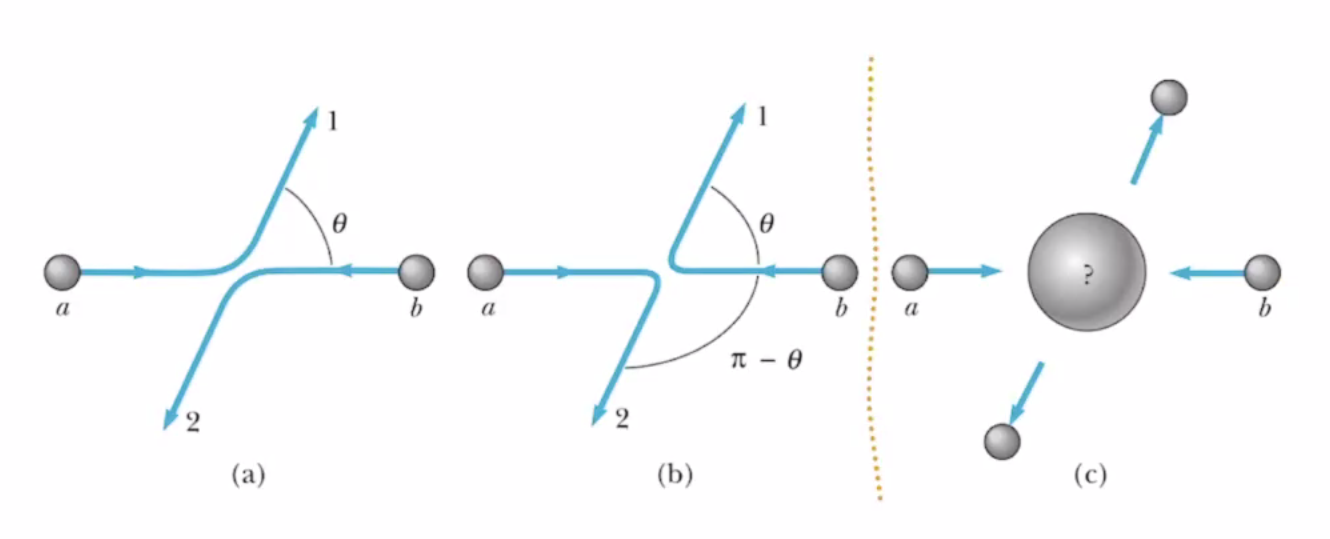
\includegraphics[width=.8\linewidth]{./Images/collision.png}
	\caption{Picture a collision of two electrons. Classical on the left. On the right, in the quantum we can't do this anymore. You don't know which outcome is the right one, because when they are interacting we can't tell which one is which due to their wave properties.}
\end{figure}

Probability density describing the probability of finding the two electrons: \\
Two-electron wave function: $ \Psi(\vec{r}, \vec{r_2}) $, where rx is the position of electron x.
$$ |\Psi(\vec{r_1}, \vec{r_2})|^2 = |\Psi(\vec{r_2}, \vec{r_1})|^2 $$

There are two options for the wave function now:
$$ \Psi(\vec{r_1}, \vec{r_2}) = \Psi(\vec{r_2}, \vec{r_1}) \rightarrow Bosons $$
$$ \Psi(\vec{r_1}, \vec{r_2}) = -\Psi(\vec{r_2}, \vec{r_1}) \rightarrow Fermions $$

``Fermions" are particles with spin 1/2: electrons, protons, neutrons, are all fermions.\\
``Bosons" are particles with integer spin: photon, Higgs boson, gluons ...

\emph{Pauli's exclusion principle applies to all ``spin 1/2" particles!}\\

\textbf{Variations of chemical and physical properties of different elements stems from how their electrons are structured:}\\
Element: Electrons,  ($n, l, m_l, m_s$)\\ 
Hydrogen:   1 electron, ground state: (1, 0, 0, $\pm 1/2$) \\
Helium: 2 electrons: (1, 0, 0, +1/2), (1, 0, 0, -1/2) \\
Lithium: 3 electrons: (1, 0, 0, 1/2), (1, 0, 0, -1/2), (2, 0, 0, $\pm 1/2$) \\

Electronic configurations follow from this principle.
\begin{figure}[h!]
	\centering
	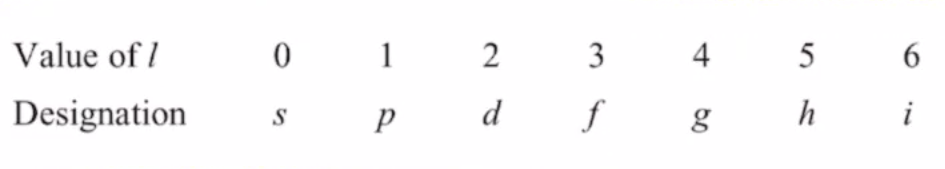
\includegraphics[width=.8\linewidth]{./Images/configurations.png}
	\caption{In a given state: max 2(2l+1) electrons. Where the first 2 is nbr $m_s$, second term nvm of $m_l$.}
\end{figure}
Hydrogen: $1s$ \\
Helium: $1s^2$ \\
Lithium: $1s^22s$ \\
. \\
. \\
. \\
Flourine: $1s^22s^22p^5$ \\

\subsection{Shells \& Subshells}
Electronic ``shells" are labeled according to their principle quantum number:

\begin{figure}[h!]
	\centering
	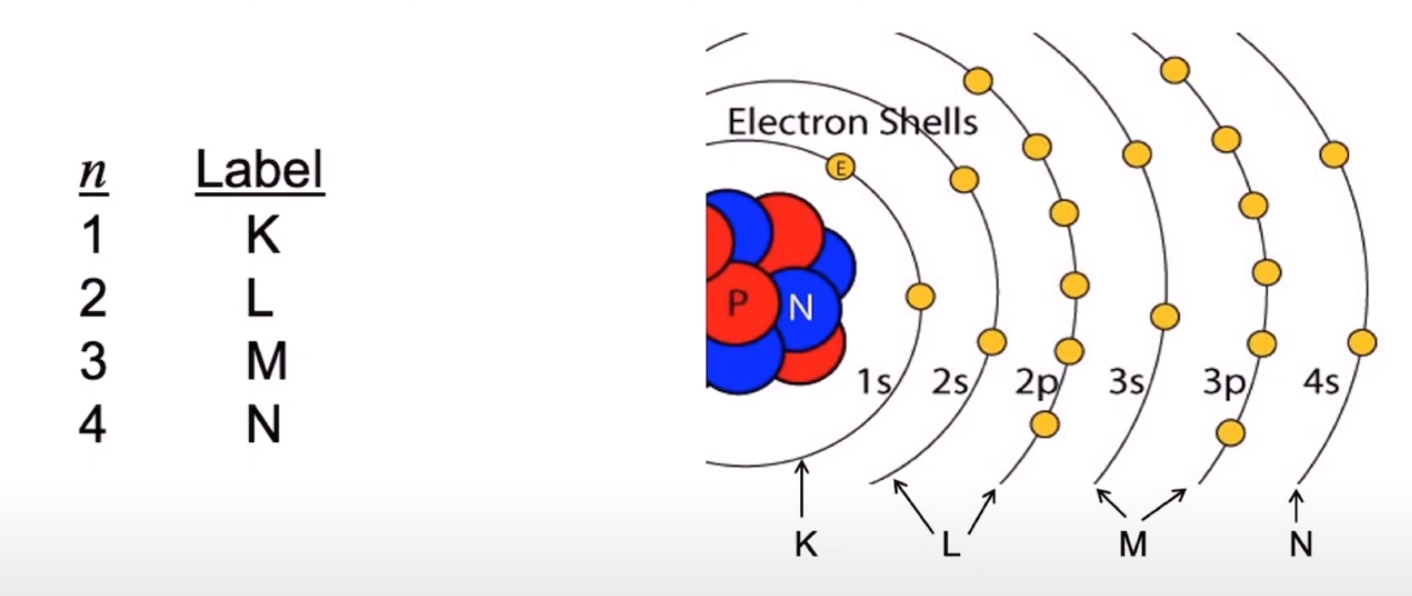
\includegraphics[width=.8\linewidth]{./Images/shells.png}
	\caption{}
\end{figure}

\textbf{Shell:} Described by principle quantum number (n)\\
\textbf{Subshell:} Described by principle quantum number (n) +
	angular momentum quantum number (l) (s, 2p, ..) \\

\subsubsection{Periodic Table and Subshells (and You!)}
Approximate filling of energy levels in many-electron systems, as the atomic number Z for the atom increases: Different subshells correspond to different energy levels.

(\emph{Note: for hydrogen atoms with a single electron, only principle
	quantum number ``n" determines the energy level. In multi-electron 
	systems, this is not the case.})

Filling ``rules":
\begin{itemize}
	\item Capacity of each subshell is 2(2l+1)
	\item Electrons occupy the lowest energy states available
\end{itemize}

\begin{itemize}
	\item An electron in the 2s level has a greater probability to be found at a small radii compared to an electron in the 2p level.
	\item Impacts ``effective" net charge that the electron ``sees" ergo.
		tighter binding of 2s electrons compared to 2p.
	\item More dominant effect for larger principle quantum number, e.g. n=4
		\begin{itemize}
			\item Tighter binding of 4s and 4p electrons results in these elctrons' energy levels being almost as low as 3d level
			\item Exact energy levels depends on the given atom!
		\end{itemize}
\end{itemize}

\begin{figure}[h!]
	\centering
	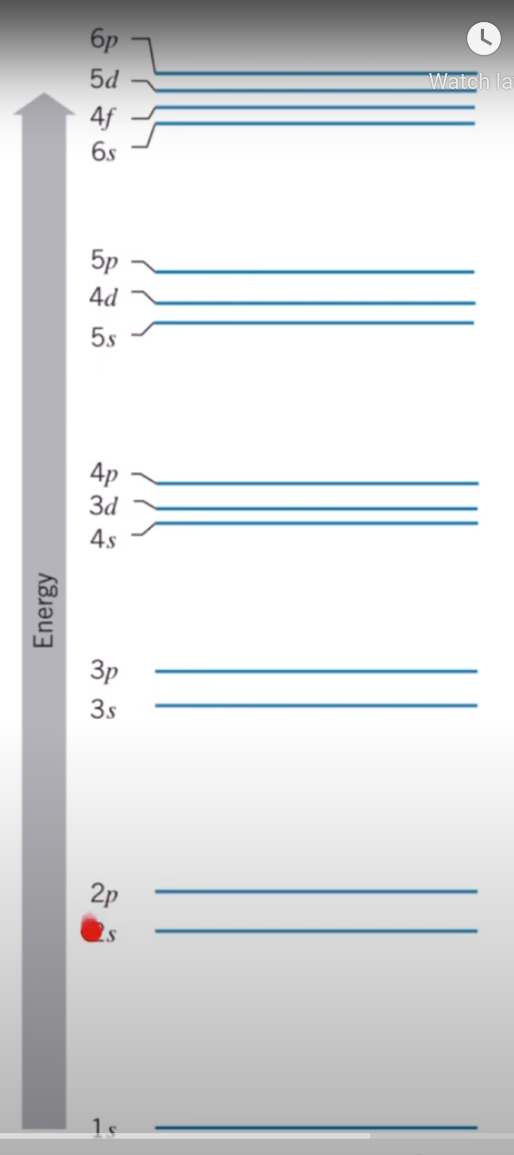
\includegraphics[width=.2\linewidth]{./Images/watch.png}
	\caption{}
\end{figure}

\newpage
\subsection{Electron Screening}

There's no simple way to calculate orbital radius for electrons in most atoms. 
Generally it's a reasonable assumption that e.g. a 2s electron is farther from the nucleus than 1s electron.\\

\begin{figure}[h!]
	\centering
	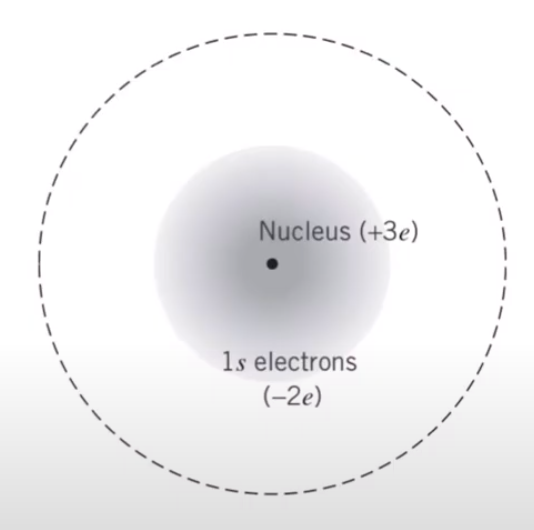
\includegraphics[width=.5\linewidth]{./Images/lithium.png}
	\caption{}
\end{figure}

\begin{result}[Effective nuclear charge]
	\emph{For an electron in 2s state:}\\
	+3e in nucleus, -2e from 1s state electrons \\
	$\rightarrow Z_{eff.} = +1e$
	Approximate estimate of energy of this level:
	$$ E_n = (-13.60 eV) \frac{Z_{eff}^2}{n^2} $$
	Li, 2s electron: $E = -3.40 eV$ \\
	Ionization of neutral lithium atom? \\
	5.39 eV (not bad).
\end{result}

This effect is called electron screening -- to an outer electron, the charge of the nucleus is ``screened" or ``shielded" by the electrons in the inner shells.\\

\emph{The less penetrating an orbit is for the outer electron, the more accurate
the above approximation is.}

\newpage
\subsection{Optical Transitions}

If an outer electron is excited to a higher energy level or removed from the atom, ``vacancy" is created an can be filled by electrons dropping in to this state.\\
Energy lost appears as emitted photons, usually have wavelengths in the visible range of the spectrum ``optical transitions".\\
Note: \\
\emph{$\Delta l = \pm 1$}\\

\section{Molecular Structure}
When atoms brought together to form molecules, atomic states of the electrons 
become molecular states.\\
Probability density of occupied molecular states determine the nature of the 
molecular bonds and the structure/properties of molecules.\\
\\

Why should molecules form at all? Coulomb potential of electrons in one atom repels electrons in another atom? \\

\emph{No, probability densities of atomic orbits are not always spherically symmetrical!}

\begin{figure}[h!]
	\centering
	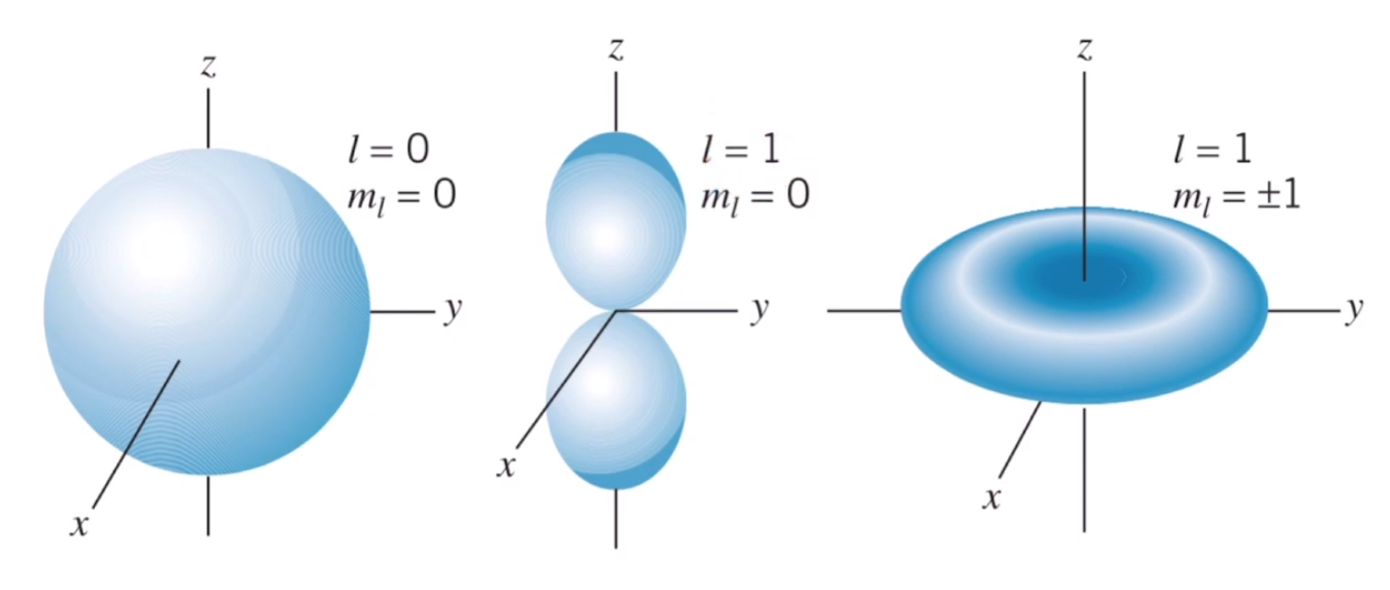
\includegraphics[width=.9\linewidth]{./Images/spherical.png}
	\caption{}
\end{figure}

\subsection{Hydrogen Molecule}
Lets start even simpler: Hydrogen Molecule Ion! $H_2^+$ \\

\begin{figure}[h!]
	\centering
	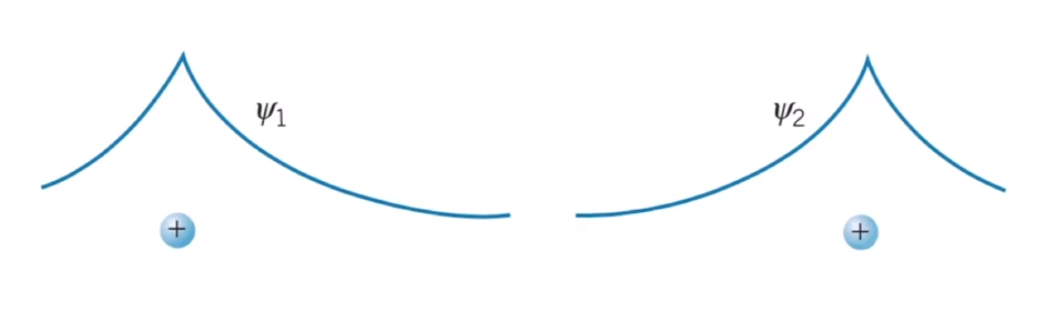
\includegraphics[width=.7\linewidth]{./Images/hydogen_molecule.png}
	\caption{Wave function for two elctrons separated by a large distance}
\end{figure}

\begin{figure}[h!]
	\centering
	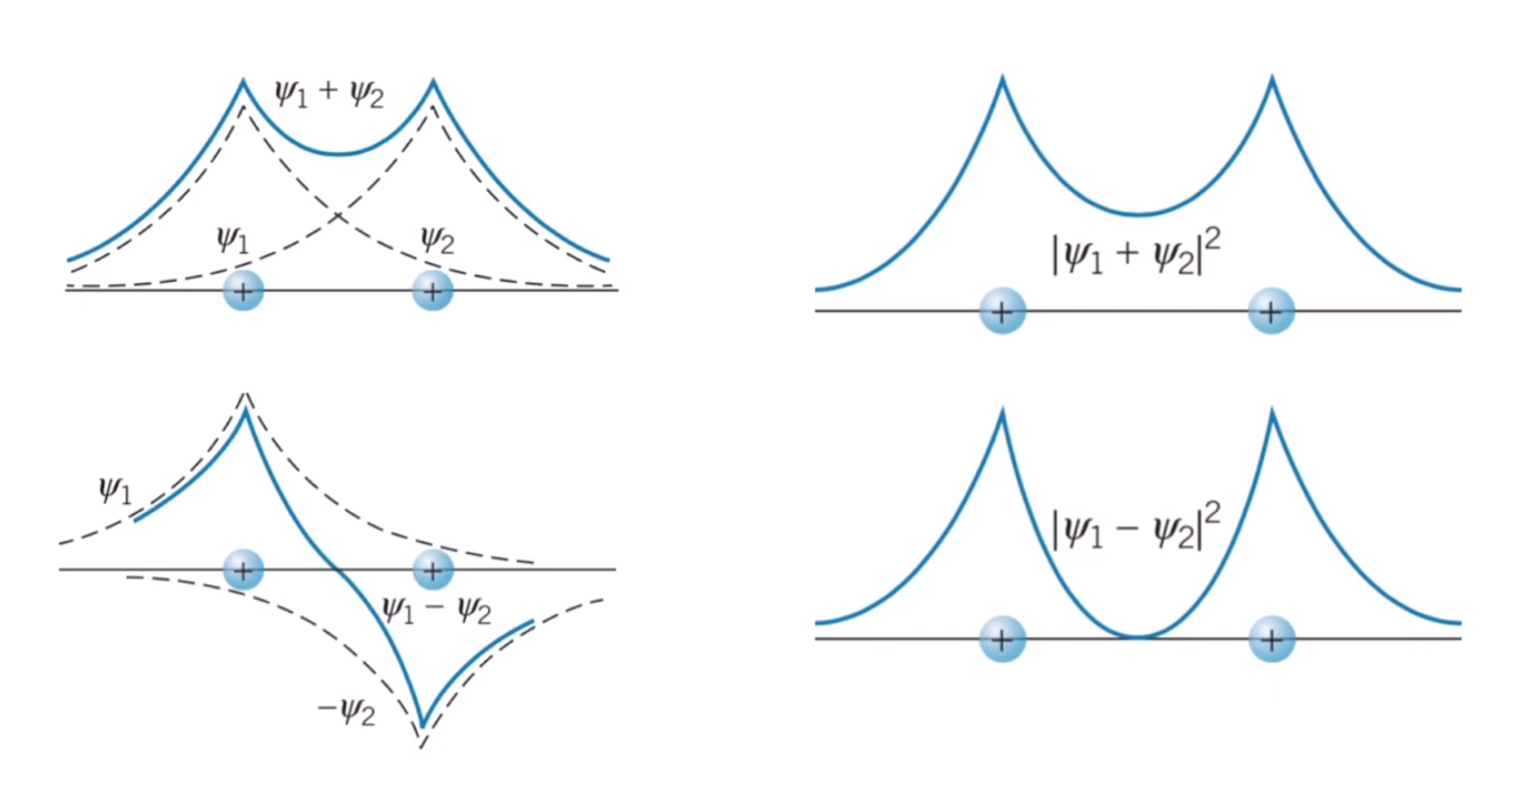
\includegraphics[width=.9\linewidth]{./Images/hydrogen_wave_functions.png}
	\caption{Left: Overlap of two wave functions. Right: Corresponding probability density}
\end{figure}

\begin{itemize}
	\item Electron is shared between the two!
	\item When the electrons are close, the wave functions begin to overlap, and we must combine them according to the rules of quantum mechanics:
		\begin{itemize}
			\item First add the wave functions
			\item Then square the wave functions to get the probability density
		\end{itemize}
	\item When combining two wave functions, relative sign matters!
\end{itemize}

Two contributions to energy of hydrogen molecule ion:

\begin{enumerate}
	\item Coulomb repulsion between the two positively charged protons
	\item Coulomb attraction between the protons and the electrons
\end{enumerate}

\emph{For stable molecules to form, total energy must be negative and the electron must provide enough negative energy of attraction to overcome the positive repulsion.}\\
\\

Generally we define molecular binding energy as energy difference between the separate components (H and H+) and the combined system, e.g.:
$$ B = E(H + H^+) - E(H_2) $$
\textbf{Molecular bonds involve sharing of a single electron between two atoms of the molecule. Electron spends most of its time between the two protons!}

\subsubsection{Continuing with hydrogen molecule...}
Molecular state that leads to a stable molecule: ``bonding state"
One state that does not lead to a stable molecule: ``anti-bonding state"

\begin{figure}[h!]
	\centering
	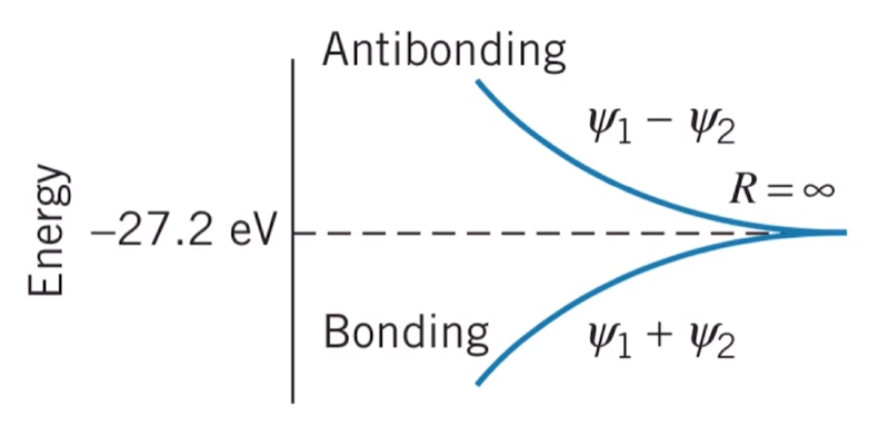
\includegraphics[width=.9\linewidth]{./Images/antibonding.png}
	\caption{}
\end{figure}

\emph{Note: for two electrons to occupy the same molecular state, their spins must be in opposite directions ergo pauli exclusion principle}

\begin{figure}[h!]
	\centering
	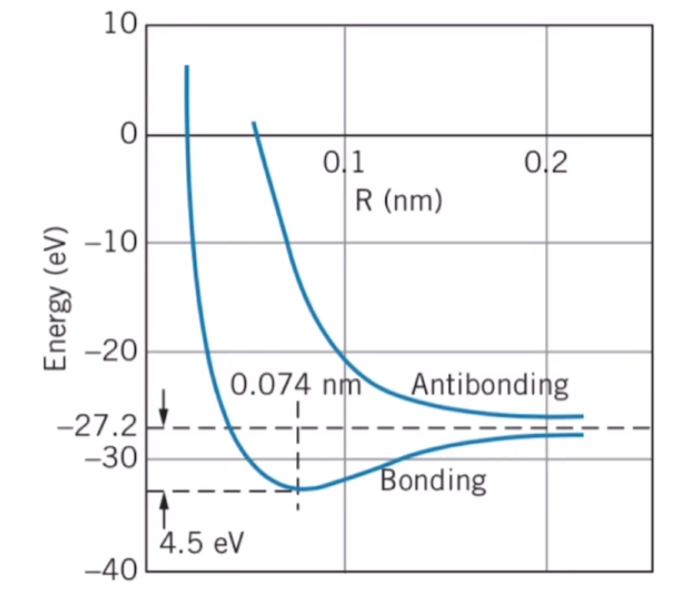
\includegraphics[width=.9\linewidth]{./Images/binding_energy.png}
	\caption{Molecular Binding Energy}
\end{figure}

\begin{question}[Molecular Binding Energy]
	$$ B = E(H + H^+) - E(H_2) $$
	$$ = 2(-13.60\ eV) - (-31.7\ eV) $$
		= 4.5 eV
\end{question}

\subsubsection{Molecules}
Forming of molecules is a tradeoff between attractive and repulsive Coulomb force. Charge is usually distributed unevenly in atoms.

\begin{figure}[h!]
	\centering
	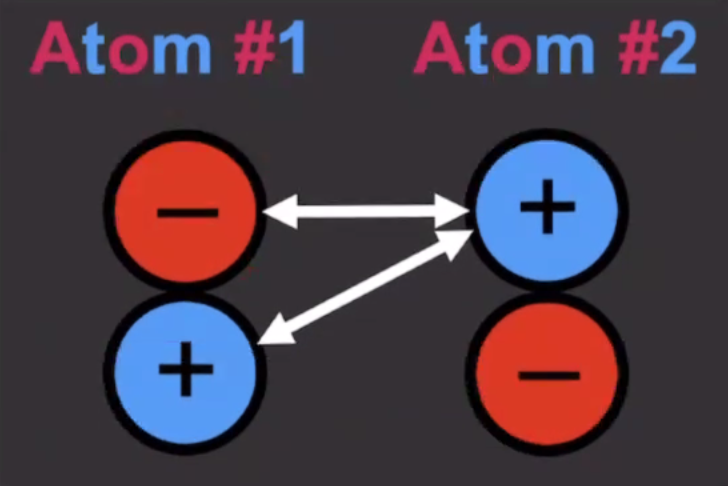
\includegraphics[width=.6\linewidth]{./Images/atom1.png}
	\caption{}
\end{figure}

\subsection{Covalent Bonding}
Common for molecules containing two identical atoms.\\
As two atoms are brought together, the electrons interact and form molecular states rather than separate atomic states:\\
For one of these, the overlap of the electron wave functions results in a lower energy than that of the separate atoms\\
For the other, anti-bonding state has an increased energy compared to the separate atoms, ergo no stable molecule.\\
Note: Pauli's principle applies to molecular states as well!\\

\subsection{Ionic bonding}
You remember this stuff, it's whatever.


\subsection{Molecular Vibrations and Rotations}
Like atoms, molecules can absorb or emit energy by changing the configuration of their electrons. \\
Molecules can also emit or absorb energy by vibrating about their equilibrium position or rotating about their center of mass.

\subsubsection{Molecular Vibrations}
Remember quantum harmonic oscillator, for oscillator in one-dimension:
$$ E_N = (N + 1/2) \bar{h}\omega\ \ \ N:\ quantum\ number,\ \omega = \sqrt{frac{k}{m}} $$

These are vibrational energies for molecules. \\

Allowed transitions for vibrational transitions (absorb or emit electromagnetic radiation):
$$ \Delta N = \pm 1 $$

\subsubsection{Vibrating Diatomic Molecules}
What is the effective mass m?\\

Consider point of motion (equilibrium point) where total energy is only kinetic energy:

$$ E_{tot} = \frac{p_1^2}{2m_1} $$
Where p1, p2 are the linear momentums of atom 1, 2.

\begin{figure}[h!]
	\centering
	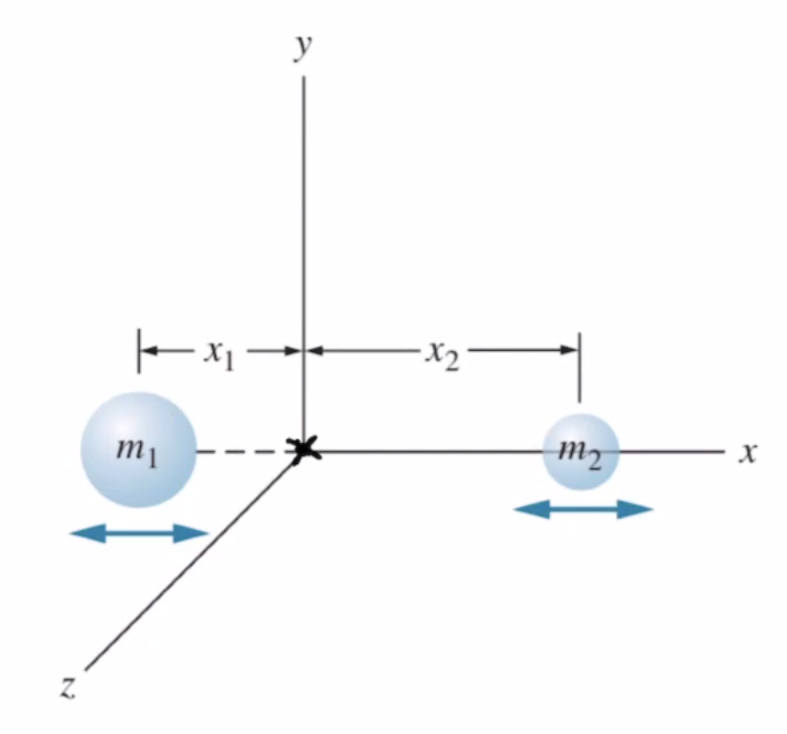
\includegraphics[width=.6\linewidth]{./Images/vibrations.png}
	\caption{}
\end{figure}

The total momentum must be zero in the reference frame of the molecule:
$$ \vec{p_1} + \vec{p_2} = 0,\ \ \ \ \ p_1 = p_2 = p $$

$$ E_{tot} = \frac{p^2}{2m_1} + \frac{p^2}{2m_2} = \frac{p^2}{2}\left(\frac{m_1 + m_2}{m_1m_2}\right) $$

Reduce ``effective" mass: $ m = \frac{m_1 + m_2}{m_1m_2}$ \\
\\

What is the effective force constant k?\\
Can be approximated by considering the motion about equilibrium position. Tabulated for different molecules (in units of $eV/m^2\ or\ N/m$).

\begin{figure}[h!]
	\centering
	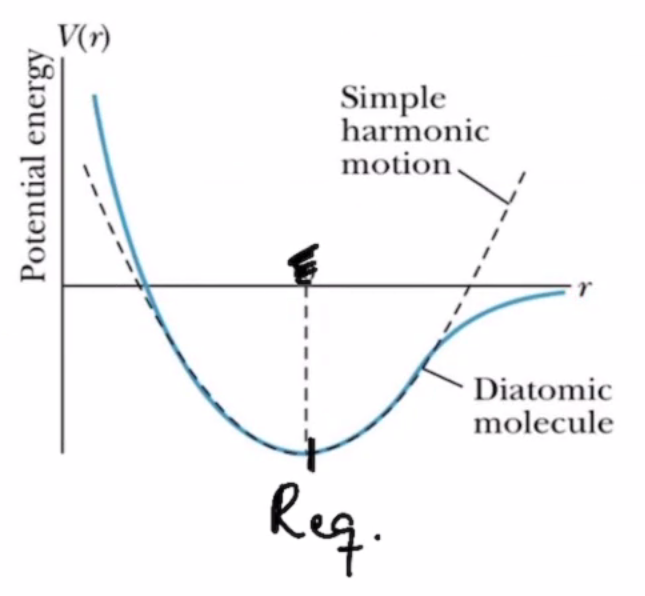
\includegraphics[width=.4\linewidth]{./Images/effective_force.png}
	\caption{}
\end{figure}

\subsubsection{Molecular Rotations}
A diatomic molecule can be thought of as two atoms held together with a massless, rigid rod. \\
In a purely rotational system, kinetic energy is expressed in terms of the rotational angular momentum (L) and rotational inertia (I).:
$$ K = \frac{1}{2} I\omega^2 = \frac{L^2}{2I} \ \ \ (From\ classical\ physics)$$

In quantum mechanics angular momentum is quantized!
$$ E_L = \frac{L(L+1)\bar{h}^2}{2I} $$
\\

Using upper case L to distinguish this angular momentum quantum number of a molecular system as opposed to lower case l representing that of a particle.\\

ALlowed transitions for rotational transitions (absorb or emit electromagnetic radiation):
$$ \Delta L = \pm 1 $$

\newpage
\subsubsection{Rotating Diatomic Molecules}
Rotational inertia of the molecule:
$$ I = m_1x_1^2 + m_2x_2^2 $$

In terms of reduced mass:
$$ m = \frac{m_1m_2}{m_1+m_2} $$

and equilibrium separation:
$$ R_{eq} = x_1 + x_2 $$

Ergo, rotational inertia:
$$ I = mR_{eq}^2 $$

Rotational energies:
$$ E_L = \frac{L(L+1)\bar{h}^2}{2mR_{eq}^2}\ \ \ l=0,1,.. $$


\begin{figure}[h!]
	\centering
	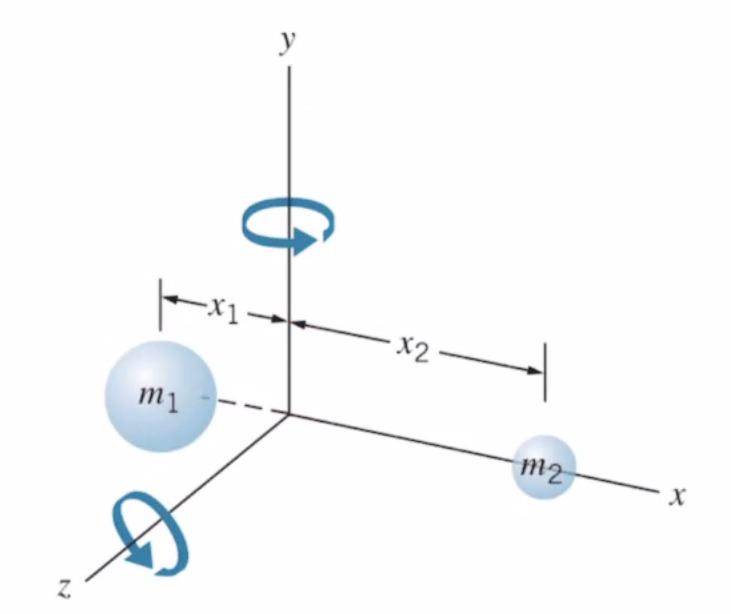
\includegraphics[width=.4\linewidth]{./Images/rotational.png}
	\caption{}
\end{figure}


\begin{figure}[h!]
	\centering
	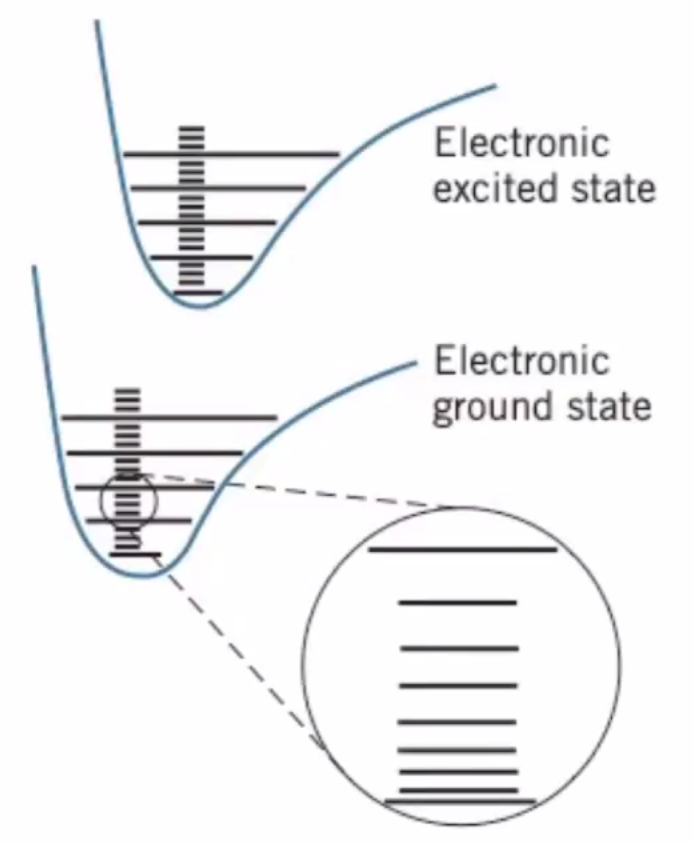
\includegraphics[width=.4\linewidth]{./Images/levels.png}
	\caption{In practice, these all combine to form different energy levels for molecules}
\end{figure}

\begin{result}[Typical size of transitions]
	\begin{itemize}
		\item Vibrational $\approx 0.1-1\ eV$
		\item Rotational $\approx 0.01-0.1\ eV$
	\end{itemize}
\end{result}

\newpage
\section{Light Amplification by Stimulated Emission of Radiation}
Lasers were first proposed by Einstien in 1917. It took nearly half a century for the first prototype to work. \\

Different ways in which radiation interact with atomic energy levels:
\begin{itemize}
	\item Spontaneous emission: When an atom in an excited state falls into a lower energy level, it emits a photon of light:
		$$ atom*\ \rightarrow atom + photon $$
	\item When at atom encounters a photon, it can absorb the photon's energy and jump to an excited state:
		$$ atom + photon \rightarrow atom* $$
	\item Stimulated emission: When a photon encounters an atom in an excited state, the photon can induce the atom to emit its energy as another photon of light, resulting in two identical photons:
		$$ atom* + photon \rightarrow atom + 2\ photons $$
\end{itemize}

\begin{figure}[h!]
	\centering
	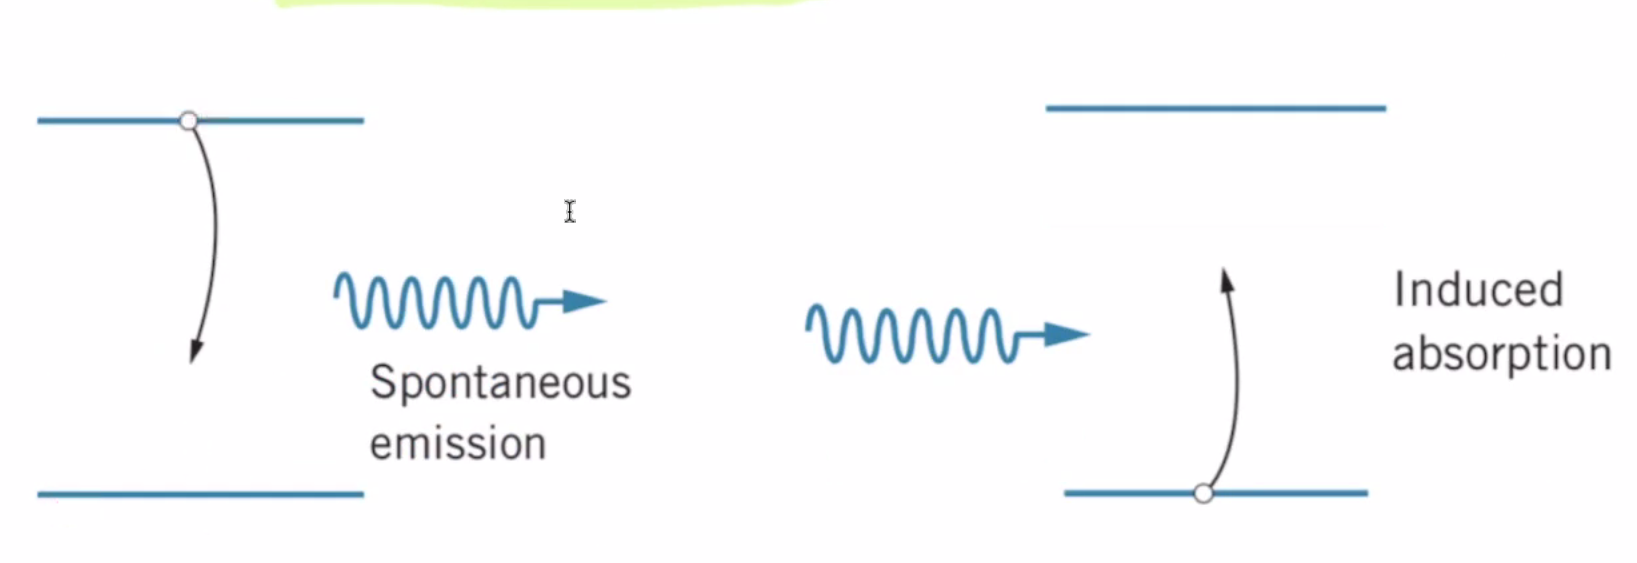
\includegraphics[width=.6\linewidth]{./Images/emission2.png}
	\caption{In practice, these all combine to form different energy levels for molecules}
\end{figure}
\begin{figure}[h!]
	\centering
	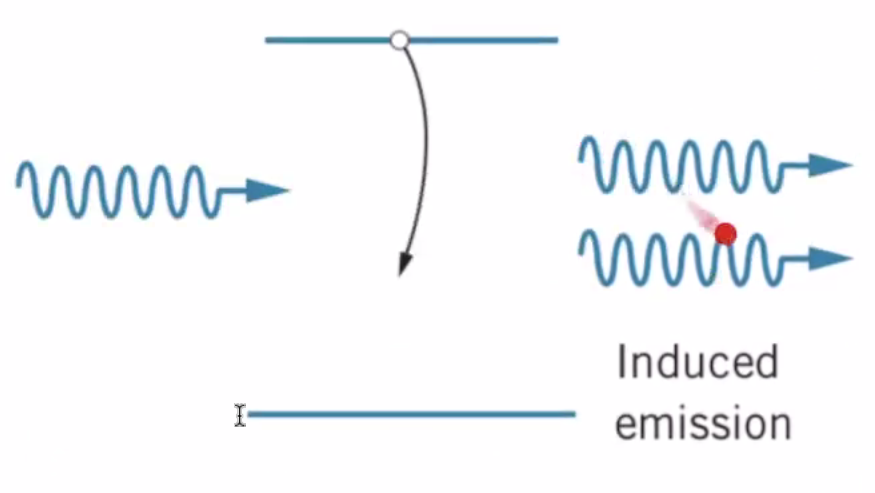
\includegraphics[width=.6\linewidth]{./Images/emission3.png}
	\caption{The two photons emerging from this proces will travel in exactly the same direction, have exactly the same direction, and be perfectly in phase.}
\end{figure}

\begin{figure}[h!]
	\centering
	\includegraphics[width=.6\linewidth]{./Images/laser.png}
	\caption{Ideal picture of the build-up of a laser beam.}
\end{figure}

Problems with this picture:
\begin{itemize}
	\item Difficult to keep a collection of atoms in an excited state
	\item Atoms back in the ground-state would undergo absorption and \emph{remove} photons
\end{itemize}

\begin{result}[Solution to 1: Population inversion]
	Atoms are ``pumped" into a very short-lived excited state which decays to a ``metastable" state (atom lives in this state for 1e-3 compared to 1e-8 in the short-lived state) \\
	By this pumping we can have more atoms in the metastable state than in the ground state. \\
	Ergo, population inversion!
\end{result}

\begin{figure}[h!]
	\centering
	\includegraphics[width=.6\linewidth]{./Images/population_inversion.png}
	\caption{Transition rule: $\Delta l = \pm 1$. A 2s electron can't decay to 1s easily.}
\end{figure}


\newpage
\begin{result}[Solution to 2: Four-level Laser]
	Atoms in the ground state are pumped to an excited state, then rapidly decay to a metastable state.\\


	The ``lasing" transition proceeds from the metastable state to another intermediate short-lived state, before the atom finally decays to the ground state.\\

	Atoms in the ground state cannot absorb photons with energy corresponding to the lasing transition!
\end{result}


\begin{figure}[h!]
	\centering
	\includegraphics[width=.6\linewidth]{./Images/four-level.png}
	\caption{T}
\end{figure}

\subsection{Helium-neon Laser}
Common example of a four-level laser. THere is a gas mixture of 90\% helium to 10\% neon. \\

Electric current pumps helium from its ground state $1s^2$ to the excited state ($1s^12s^1$). This is metastable, since transition is forbidden.\\

\begin{figure}[h!]
	\centering
	\includegraphics[width=.6\linewidth]{./Images/helium-neon.png}
	\caption{T}
\end{figure}

Occasionally, excited helium atom will collide with ground-state neon atom. Excited atom yadda yadda.

\begin{figure}[h!]
	\centering
	\includegraphics[width=.6\linewidth]{./Images/schematic_of_laser.png}
	\caption{T}
\end{figure}

Typical helium-neon lasers have a very low efficiency. However, it is useful because it has high coherence and directionally and its energy density is very high.

\begin{figure}[h!]
	\centering
	\includegraphics[width=.6\linewidth]{./Images/lasers_rock.png}
	\caption{T}
\end{figure}

There are many applications of lasers but of course, bar-code scanners, laser-printers, LiDAR.

\section{Bonding in solids}
A crystalline solid consists of a large number of atoms arrange din a regular array, forming a periodic structure. This structure is called a lattice.\\

Bonding schemes for molecules are also appropriate for describing the bonding mechanisms in solids, e.g.
\begin{itemize}
	\item Ions in the NaCl are ionically bonded
	\item Carbon atoms in the diamond structure form covalent bonds
	\item Van der Walls bonding is responsible for cohesion of organic solids in yadda fml
\end{itemize}

\subsection{Ionic Solids}

Dominant effect is the Coulomb interaction, creating a net attractive potential energy due to all the interactions:
$$ U_c = - \alpha \frac{e^2}{4\pi\epsilon_0} \frac{1}{R} $$
$\alpha$: Madelung constant\\
R: Distance between two adjacent ions \\

Madelung constant depends on the geometry of the lattice. \\

For NaCl is an fcc:
$\alpha = 1.7476$

For CsCl is an bcc:
$\alpha = 1.7627$

There is also a repulsive potential energy due to Pauli exclusion principle:
$$ U_R = AR^{-n} $$
A: Strength of potential energy \\
n: How rapidly it increases for smaller R \\

The total potential energy per ion pair of the crystal:
$$ U_{total} = U_c + U_R = -\alpha \frac{e^2}{4 \pi \epsilon_0} \frac{1}{R} + AR^{-n} $$

THe potential energy has a minimum ($U_0$) called ionic cohesive energy at the equilibrium separation ($R_0$).
$$ U_0 = \frac{-\alpha e^2}{4\pi\epsilon_0 R_0} \left(1 - \frac{1}{n} \right) $$

Binding energy: B = $-U_0$.

\begin{figure}[h!]
	\centering
	\includegraphics[width=.8\linewidth]{./Images/tabulated.png}
	\caption{Tabulated measured values for different ionic crystals. Listed molar cohesive energy related to above minimum potential energy as: $E_{coh.} = -U_0 \cdot N_A = B \cdot N_A$}
\end{figure}

\subsection{Covalent Solids}
Specifically, diamond.

\begin{itemize}
	\item Atomic carbon electron configuration: $1s^22s^22p^2$
	\item Each carbon atom in diamond bonds covalently to four other carbon atoms to form a stable closed-shell structure - basic structure of diamond is called tetrahedral
	\item Atomic cohesive energies are generally greater than in ionic solids
\end{itemize}

\begin{figure}[h!]
	\centering
	\includegraphics[width=.8\linewidth]{./Images/covalent.png}
	\caption{}
\end{figure}

\begin{figure}[h!]
	\centering
	\includegraphics[width=.8\linewidth]{./Images/tetrahedral.png}
	\caption{}
\end{figure}

\subsection{Metallic Solids}
Metallic bonds are generally weaker than ionic or covalent bonds. The valence electrons in a metal are relatively free to move throughout the material. The binding mechianism in a metal is the attractive force between yadda fml.

\newpage
\begin{question}[Ionic Solids]
	Determine the experimental value of the binding energy of an ion pair in the NaCl lattice from the cohesive energy.
	\begin{answer}[A]
		Binding energy $B = \frac{E_{coh}}{N_A}$ \\
	$$ = \frac{769 \cdot 10^3 J/mol}{6.02 \cdot 10^{23} ions/mol} \approx 7.98 eV $$
	\end{answer}

	Find the expected value of the binding energy based on the lattice parameters.
	\begin{answer}[B]
		Binding energy from minimum potential energy:
		$$ B = -U_0 = \frac{\alpha e^2}{4\pi \epsilon_0 R_0} \left(1-\frac{1}{n}\right) $$
		The constants are 1.44 eV nm and 1.7476. So we get
		$$ 1.44\ eV \cdot nm \cdot 1.7476 /0.281 nm \cdot (1-1/9) $$
		$\approx 7.96 eV$
	\end{answer}

	These two answers end up being almost exactly identical!
\end{question}

\section{Statistical Physics Detour}
Satistical physics deals with the distribution of a fixed amount of energy among a number of particles that are identical and indistinguishable in any way (quantum particles). The probability of finding particles in a given energy state is called a ``distribution function". For quantum particles, these probabilities are very different for ``fermions" (particles of spin 1/2 like electrons), and ``bosons" (particles with integer spin, like photons). 
\begin{itemize}
	\item Bose-Einstein distribution - Describes bosons. No limit on number of particles in a given energy state.
	\item Fermi-Dirac distribution - Describes fermions. No more than one particle per quantum state allowed.
\end{itemize}


\begin{figure}[h!]
	\centering
	\includegraphics[width=.8\linewidth]{./Images/fermi-dirac.png}
	\caption{F(E). $E_F$: Fermi energy}
\end{figure}

\subsection{Electrons in Metals and Conduction}
In metals, each atom contributes one or more loosely bound electrons to an ``electron gas". 
\begin{itemize}
	\item Shortly after discovery of the electron, Drude and Thomson proposed the ``free electron theory" of metals to explain the physical properties of a metal.
	\item Models metal as a classical gas of conduction electrons through a fixed lattice of positive ions (used to explain electrical and thermal conductivities).
\end{itemize}

\begin{result}[Ohm's Law]
	$$ \vec{j} = \sigma \vec{E} $$
	Where: \\
	E is electric field (V/m) \\
	sigma is electrical conductivity (1/Omega m) \\
	j is current density (A/m/m) \\
	\\

	This was first an experimental result, applicable to different metals and semiconductors. It states that current density in a meterial is directly proportional to the applied electric field.
\end{result}

One can actually derive Ohm's law by considering a conductor to consist of a gas of classical particles moving through a background of immobile, heavy ions.

\begin{figure}[h!]
	\centering
	\includegraphics[width=.8\linewidth]{./Images/ohms.png}
	\caption{}
\end{figure}

Free electrons in the electron gas experience a force:
$$ \vec{F} = -e \vec{E} $$

... and corresponding acceleration:
$$ \vec{a} = \frac{\vec{F}}{m_e} = \frac{-e \vec{E}}{m_e} $$

Acceleration of electrons is countered by collisions, net result is that electrons acquire a steady ``drift velocity" ($\vec{v_d}$), given by acceleration x average time between collisions ($\tau$):
$$ \vec{v_d} = \vec{a} \tau = \frac{-e\vec{E}\tau}{m_e} $$

Magnitude of current density is determined by number of charge carriers and their average speed:
$$ \vec{j} = -ne\vec{v_d} = \frac{ne^2\tau}{m_e}\vec{E} $$
Note: $\tau = l/v_{av}$ \\ 
Where l = mean free path and $v_{av}$ = average speed of electrons in the lattice.\\

Nice! Electron gas model predicts Ohm's law. However, it results in conductivity values that differ from measured values by an order of magnitude... \textbf{quantum effects were ignored!} \\

Must use Fermi-Dirac distribution for the conduction electrons in the metal.\\ 
Must take the wave nature of the electron into account in calculating the electron ``mean free path".\\

\subsection{Band Theory of Solids}

What happens if you have two atoms that you bring together?
\begin{itemize}
	\item Two sodium atoms, each having an outermost 3s electron with a specific energy
	\item As the two sodium atoms are brought closer together, their wave functions overlap, and the two degenerate, isolated 3s energy levels are split into two different levels.
\end{itemize}

\begin{figure}[h!]
	\centering
	\includegraphics[width=.8\linewidth]{./Images/add_or_subtract.png}
	\caption{When the wave functions add, we have a sizeable probability between the two atoms, whereas when they subtract we have a low probability between the two atoms.}
\end{figure}

When a large number of atoms are brought together, a similar phenomenon occurs. As the atoms are brought close together, the various isolated-atom energy levels begin to split.

\begin{figure}[h!]
	\centering
	\includegraphics[width=.8\linewidth]{./Images/crop.png}
	\caption{}
\end{figure}

All atoms in a solid:\\
Considering all atoms in a solid gives a very large number of levels (determined by N) spaced within the width $\Delta E$. These levels can be regarded as a \emph{continuous} band of energy levels.\\

\textbf{Energy bands in sodium metal:}
Sodium is a good electrical conductor, the 3s band is only half-filled. Large variation in electrical conductivity of metals, insulators, and semiconductors can be explained qualitatively in terms of energy bands.

\begin{figure}[h!]
	\centering
	\includegraphics[width=.4\linewidth]{./Images/bands.png}
	\caption{}
\end{figure}

\subsection{Conduction in Metals vs Insulators vs Semiconductors}
\subsubsection{Conduction in metals}
If an electric field is applied to the metal... electrons with energies near the Fermi energy can gain a small amount of additional energy from the field and reach nearby empty energy states. \\

i.e. Electrons are free to move only a small applied field in a metal due to many unoccupied energy states very close to occupied energy states == good conductor.

\begin{figure}[h!]
	\centering
	\includegraphics[width=.8\linewidth]{./Images/metals.png}
	\caption{}
\end{figure}

\subsubsection{Conduction in Insulators}
Although an insulator has many vacant states in the conduction band that can accept electrons, there are so few electrons actually occupying conduction band that can accept electrons, there are so few electrons actually occupying conduction-band states at room temperature.\\

Separation between outermost filled and empty bands referred to as the ``energy gap" of the material. Lower band filled with electrons is the ``valence band" and upper, empty band is the ``conduction band".

\subsubsection{Conduction in Semiconductors}
Semiconductors are materials that have a smaller energy gap ($<1$ eV). At T ~0 K all electrons are in the valence band. At ordinary temperatures, a sizable number of electrons are thermally excited from the valence to the conduction band.

\begin{itemize}
	\item Many empty nearby states in the conduction band implies small applied potential can easily raise the energy of the electrons in the conduction band, resulting in a moderate current.
	\item Because thermal excitation across the narrow gap is more probable at higher temperatures, the conductivity of semiconductors depends strongly on temperature.
\end{itemize}

\begin{figure}[h!]
	\centering
	\includegraphics[width=.8\linewidth]{./Images/in_summary.png}
	\caption{}
\end{figure}

\subsection{Back to Sodium}


\begin{figure}[h!]
	\centering
	\includegraphics[width=.8\linewidth]{./Images/band_cont.png}
	\caption{As we add more and more sodium atoms together, energy levels of the combined system split further and further, until the nergy difference between distinct levels is so small it cannot be distinguished.}
\end{figure}

For a single sodium atom: 3s level is half full (1 electron, max 2 allowed).
For a sodium solid: 3s band is half full (N electrons in the band, max 2N allowed).

\subsection{Bands}
Large variation in electrical conductivity of metals, insulators, and semiconductors can be explained qualitatively in terms of energy bands.

\subsubsection{Metals}
Metals have partialy filled energy bands. As a result, there are many unoccupied energy states very close to occupied energy states. Electrons can therefore easily move through the metal, with only a small applied electric field. They are good conductors.

\begin{figure}[h!]
	\centering
	\includegraphics[width=.8\linewidth]{./Images/metal_band.png}
	\caption{}
\end{figure}

\subsubsection{Insulators}
Have a lower completely filled band (valence band) and an upper completely empty band (conduction band). These are separated by a larte energy gap, which is so large that electrons effectively cannot get thermally excited to the conduction band. The electrons cannot move, and it does not conduct. 

\begin{figure}[h!]
	\centering
	\includegraphics[width=.8\linewidth]{./Images/insulator_band.png}
	\caption{}
\end{figure}

\subsubsection{Semiconductors}

SMaterial with a small energy gap, such that some electrons are thermally excited to the conduction band where they can move. Many empty nearby states, therefore small applied electric field can easily raise the energy of electrons inthe conduction band, resulting in a moderate current. They are decent conductors at room temperatures.

\begin{figure}[h!]
	\centering
	\includegraphics[width=.8\linewidth]{./Images/semiconductor_band.png}
	\caption{}
\end{figure}

\subsubsection{More Complicated Band Structures}

Why is magnesium a good conductor? Magnesium atom: $1s^22s^22p^63s^2$ (filled outer shell). \\
Why is carbon a good conductor? Magnesium atom: $1s^22s^22p^2$ (filled outer shell).

\begin{figure}[h!]
	\centering
	\includegraphics[width=.8\linewidth]{./Images/complicated_band.png}
	\caption{In Magnesium, the 3p and 3s levels overlap so it's easy to excite. In carbon, there's actually a full band and a large energy gap up to the next four levels, because crazy reasons??}
\end{figure}

\subsection{Conduction in Semiconductors}
\subsubsection{Holes}
When electrons move into the conduction band, they leave behind vacancies in the valence band. These vacancies are called holes.

Because holes represent the absence of negative charges, it is useful to think of them as positive charges.

Electrons move in a direction opposite to the applied electric field, the holes move in the direction of the electric field.

\begin{figure}[h!]
	\centering
	\includegraphics[width=.8\linewidth]{./Images/holes.png}
	\caption{}
\end{figure}

\subsubsection{Intrinsic Semiconductors}

A semiconductor in which there is a balance between the... number of electrons in the conduction band, and the number of holes in the valance band..  is called an intrinsic semiconductor.

\begin{figure}[h!]
	\centering
	\includegraphics[width=.8\linewidth]{./Images/intrinsic.png}
	\caption{Covalent bonding in Si or Ge, with each atom providing four electrons for covalent bonds with its neighbors.}
\end{figure}

\begin{figure}[h!]
	\centering
	\includegraphics[width=.8\linewidth]{./Images/intrinsic2.png}
	\caption{Another illustration of conduction in an intrinsic semiconductor.}
\end{figure}

\subsubsection{Impurities and Doping}

Both the type and number of carriers in a semiconductor may be tailored to the needs of a particular device by the addition of specific impurities in a process called doping. For example, conductivity can be increased through small amount of impurity added. These materials are called ``extrinsic" semiconductors or ``impurity" semiconductors (or ``doped" semiconductors).

\begin{figure}[h!]
	\centering
	\includegraphics[width=.8\linewidth]{./Images/replace.png}
	\caption{Example: Replace a Si/Ge atom with a valence-5 atom(left) or a valence-3 atom(right)}
\end{figure}

Resulting energy levels formed by valence-5 impurities are known as ``donor states" and a semiconductor that has beendoped with donor impurities is a ``n-type" semiconductor. (Conductivity mostly due to negative electrons).\\

Resulting energy levels formed by valence-3 impurities are known as ``acceptor states" and a semiconductor that has been doped with donor impurities is a ``p-type" semiconductor. (Conductivity mostly due to positively charged holes).\\

\begin{figure}[h!]
	\centering
	\includegraphics[width=.8\linewidth]{./Images/doping.png}
	\caption{Note: both are electrically neutral, since made of neutral atoms!}
\end{figure}

\subsection{Diodes}
Little energy is needed for eelctrons in donor states to enter the conduction band, or for electrons from valence bands to fill acceptor states and give positively charged holes in the valence band.

Region between the two material is known as depletion region as it is largely depleted of charge carriers. In equilibrium, enough negative charge biulds up in the p-type region to stop further any flow of electrons. There is a net electric field blah.

\subsubsection{Diode: Forward-bias configuration}
Connect positive side of battery to p-type material. Depletion region is narrowed and potential energy difference across p-n junction is reduced. Electrons (holes) flow easily.

\subsubsection{Diode: Reverse-bias configuration}
Connect positive side of battery to n-type material. Depletion region is widened and potential energy difference across p-n junction is increased. Few or none of the electrons can climb the potential barrier - no current.

\begin{figure}[h!]
	\centering
	\includegraphics[width=.8\linewidth]{./Images/diode.png}
	\caption{}
\end{figure}

\subsection{Transistor}
Transistors are devices that amplify coltages or currents in many kinds of circuits. The first transistor was developed in 1948 and revolutionized society. An example of a junction transistor consists of a semiconducting material with a very narrow n-type region sandwiched between two p-type regions, called the pnp transistor.

\begin{figure}[h!]
	\centering
	\includegraphics[width=.4\linewidth]{./Images/pnp.png}
	\caption{Junction Transistor}
\end{figure}

\newpage
\section{Nuclear Physics}

\subsection{Nuclear Size and Shape}
Nuclei lack a hard surface or easily definable radius. The density of the nucleus is rather uniform, and does not depend much on the mass number A.

$$ \frac{\# neutrons\ +\ protons}{volume\ of\ nucleus} = \frac{A}{4/3\ \pi R^3} \approx constant $$

\begin{figure}[h!]
	\centering
	\includegraphics[width=.6\linewidth]{./Images/nuclear_radius.png}
	\caption{}
\end{figure}

\begin{result}[Nuclear Radius]
	$$ R = R_0 \cdot A^{1/3} $$
	$R_0$ is a constant from experiments, $\approx 1.2\ fm$.
\end{result}

\begin{question}[What is the density of a typical nucleus?]
	$$ \sigma = \frac{m}{V} \approx \frac{A \cdot m_p}{4/3 \pi r^3} = \frac{A \cdot m_p}{4/3\ \pi R^3_0(A^{1/3})^3} = \frac{m_p}{4/3\ \pi R_0^3} $$
	$$ \frac{\approx 1.67 \cdot 10^{-27} kg}{4/3\ \pi (1.2 \cdot 10^{-15}\ m)^3} $$
	$$ \sigma \approx 2 \cdot 10^{17} kg/m^3 $$
	Compare to density of water, 1000 $kg/m^3$.... 14 orders of magnitude larger!!!
\end{question}

\subsection{Nuclear Mass and Binding Energy}
The nuclear binding energy is calculated as the difference between the rest energy of the consituents and the rest energy of their combination. \\

For a nucleus X with mass number A and Z protons + N neutrons: $\ce{^A_ZX_N}$
$$ B = \left( N \cdot m_N + Z \cdot m(\ce{^1_1H_0}) - m(\ce{^A_ZX_N})\right) c^2 $$

We use atomic masses rather than nuclear masses (allows using tabulated atomic masses)! Electron masses cancel out in this expression! Binding energy of electrons is in comparison very, very small -- can safely be ignored.

\newpage
\subsubsection{Binding Energy Per Nucleon}
B/A = Total binding energy/number of nucleons (protons + neutrons (A = Z + N))

\begin{figure}[h!]
	\centering
	\includegraphics[width=.6\linewidth]{./Images/binding_per_nucleon.png}
	\caption{Iron is the most stable nucleus. After which, the binding energy per nucleon begins to decrease, due to increasing Coulum repulsion. The decrease we observe for low mass number elements can be explained by surface area - more balls are sticking out relative to the size of the nucleus itself.}
\end{figure}

\subsubsection{Separation Energies}
Ionization energy is the smallest amount of energy necessary to remove an electron from an atom. \\
This typical scale is in the order of eV. \\
The Proton/neutron separation energy by contrast is the energy required to remove the least bound proton/neutron from the nucleus.
This typical scale is in the order of MeV. \\

\subsection{Nuclear Force}
The nuclear force is the strongest of known forces, also called the ``strong force". (The four fundamental forces of nature are):
\begin{enumerate}
	\item Gravitational interaction
	\item Weak interaction
	\item Electromagnetic interaction
	\item Strong interaction
\end{enumerate}

It has a very short range -- acts over distances of about 1 fm. Compare how nuclear density was about constant - it's like a nuclear force is acting between nucleons that are touching each other. \\

Nuclear force does not depend on whether nucleons are protons or neutrons. \\

It's like a spring - at a certain point it snaps then does nothing.

\subsection{Stable Nuclei and Radioactive Decays}

\begin{figure}[h!]
	\centering
	\includegraphics[width=.6\linewidth]{./Images/stable.png}
	\caption{The blue line is the line where N = Z. The blue band is made up of different stable nuclei, while the larger grey band is made up of all known nuclei, which are radioactive. The known nuclei does not follow the N=Z line - only at low N. As we go higher, due to increasing Coulomb repulsion, we need more neutrons.}
\end{figure}

Most nuclei are unstable -- they decay into lighter, more stable nuclei.

\subsubsection{Different Decay Processes}

\begin{itemize}
	\item \textbf{Alpha Decay:} Emission of a helium nucleus. \\
		$$ \ce{^A_ZX} \rightarrow \ce{^{A-4}_{Z-2}X^1} + \ce{^4_2He} $$
		\begin{question}[What is the alpha decay chain of 226-radium?]
			$$ \ce{^{226}_{88}Ra} \rightarrow \ce{^{222}_{86}Rn} + \ce{^4_2He} $$
		\end{question}
	\item \textbf{Beta Decay:} they do stuff too??
	\item \textbf{Gamma Decay:}
\end{itemize}

\subsubsection{Activity and Decay Probabilities}

Rate at which unstable nuclei decay is called the ``activity". \\

We measure activity in units of 1 becquerel (Bq) = 1 decay/second \\
We measure activity in units of 1 curie (Ci) = $ 3.7 \cdot 10^{10} $ decays/second \\

Decay probability per nucleus per second is called the ``decay constant" ($\lambda$). It is assumed to be constant with time for a particular material, i.e. the probability is independent of age of sample.

\begin{result}[Relationship between activity and decay constant]
	$ a = \lambda N $ Where N=number of nuclei.
\end{result}

\begin{result}[Exponential law of radioactive decay]
	Activity $a = - \frac{dN}{dt} $
	$$ \lambda N = - \frac{dN}{dt}\ \ or\ \frac{dN}{N} = -\lambda\ dt $$
	$$ N = N_0 e^{-\lambda t} $$
	Where $N_0$: number of nuclei at t=0.
	Usually we cannot measure N, but we can express this in terms of activity instead, which is easier to measure.

	$$ a = a_0 e^{-\lambda t} $$
	Where $a_0$ is the original activity at t=0.
\end{result}

ALso talk about the ``half-life" of the decay, the time for activity to be reduced by half:

$$ t_{1/2} = \frac{1}{\lambda} ln(2) \approx \frac{0.693}{\lambda} $$

The mean lifetime:

$$ \tau = \frac{1}{\lambda} $$

\begin{figure}[h!]
	\centering
	\includegraphics[width=.6\linewidth]{./Images/decay.png}
	\caption{}
\end{figure}

\subsection{Alpha Decay}
Alpha decay involves disintegrating an unstable nucleus into a lighter nucleus and alpha particle. \\

The energy released (Q) through this process appears as kinetic energy (K) of the alpha particles and ``daughter" nucleus (assume initial atom X at rest):

$$ Q = \left( m(x) - m(x') - m(\ce{^4_2He})\right)c^2 $$
$$ Q = K_{x'} + K_\alpha $$
Also:
$$ P_{x'} = P_{alpha} $$

Where
$$ K = \frac{P^2}{2m} $$

\begin{figure}[h!]
	\centering
	\includegraphics[width=.6\linewidth]{./Images/alpha_decay.png}
	\caption{}
\end{figure}

Both energy and linear momentum must be conserved in this process:
$$ K_{\alpha} \approx \frac{A-4}{A} Q $$

\subsection{Beta Decay}
Beta decay involves a neutron transforming into a proton or vice-versa. One may think that the process as $n \rightarrow p + e^-$, but this has problems. \\

This would violate conservation of angular momentum (spin!)\\
Measurements of energy of emitted electrons showed a continuous spectrum of emitted energies rather than the expected value.
\begin{figure}[h!]
	\centering
	\includegraphics[width=.6\linewidth]{./Images/unexpected.png}
	\caption{There is a distribution instead of a single value as expected.}
\end{figure}

$$ Q = \left(m_n - m_p - m_e \right)c^2 \approx 0.78 MeV $$

Solution: There is a third particle involved!! \\
$ Neutrino:\ \nu$\\
$ Antineutrino:\ \vec{\nu}$

Neutrinos: zero electric charge, teensy mass, spin 1/2.\\

Neutron decay: $n \rightarrow p + e^- + \vec{\nu}$, $\tau(n) \approx$ 14 min 40 sec. \\

Beta decay of neutron in a nucleus:
$$ \ce{^A_ZX} \rightarrow \ce{^A_{Z+1}X'} + e^- + \vec{\nu} $$

Protons in some nuclei can also undergo beta decay: 
$$ p \rightarrow n + e^+ \nu\ Where\ e^+\ is\ a\ positron. $$
$$ \ce{A_ZX} \rightarrow \ce{^A_{Z-1}X'} + e^+ + \nu $$
Fortunately, this cannot happen for a free proton because it requires energy. \\\\

Proton beta decay is never observed for free protons. 

\begin{figure}[h!]
	\centering
	\includegraphics[width=.6\linewidth]{./Images/universe.png}
	\caption{The expected lifetime of a proton is $10^{34}$ years. Which is many many many orders of magnitude longer than the age of the universe.}
\end{figure}






\end{document}
